%Nesta seção será apresentada toda a evolução da automação. Além disso serão explicados todos os conceitos necessários para a compreensão deste projeto. Também será exposto o porquê é necessário a execução deste projeto de trabalho de conclusão de curso dentro do curso de Engenharia Elétrica da UFSM-CS. \textcolor{red}{(Atualizar)}
\section{Brasil e seu mapa eólico}
\par As energias renováveis têm ganhado destaque no cenário energético mundial devido à urgência de mitigar as mudanças climáticas e reduzir as emissões de gases de efeito estufa. No Brasil, o potencial para a adoção de energias renováveis é vasto, dado seu território extenso e condições climáticas favoráveis. Entre as fontes renováveis, a energia eólica se destaca como uma das mais promissoras, contribuindo significativamente para a matriz energética do país.
\par O desenvolvimento da energia eólica no Brasil começou a se intensificar no início dos anos 2000, impulsionado por políticas públicas e incentivos governamentais. O \citeonline{proinfa2024}, lançado em 2002, foi um marco inicial, proporcionando contratos de compra de energia de longo prazo que atraíram investidores. A partir de 2009, a realização de leilões específicos para fontes renováveis, incluindo a eólica, promoveu uma expansão acelerada do setor, tornando a energia eólica uma das fontes mais competitivas no Brasil.
\par O Brasil rapidamente se tornou um dos maiores mercados para energia eólica no mundo. A capacidade instalada de energia eólica passou de menos de 1 GW em 2009 para mais de 20 GW em 2023, como destacado nas Figuras \ref{fig:Turbinas_instaladas} e \ref{fig:evolucaoCapacidadeInstalada}. Este crescimento foi suportado pela combinação de políticas públicas favoráveis, avanços tecnológicos, e a competitividade econômica da energia eólica.

\begin{figure}[H]
    \caption{Crescimento da geração de Energia Elétrica oriunda da Energia Eólica.}
    \label{fig:Turbinas_instaladas}
    \centering
    \includegraphics[width=0.8\textwidth]{Figuras/Teorico/PotencialEólico_ParquesInstalados.png}
    \fonte{\citeonline{abeeolica2017}}
\end{figure}

\begin{figure}[H]
    \caption{Evolução da Capacidade Instalada de Energia Eólica}
    \label{fig:evolucaoCapacidadeInstalada}
    \centering
    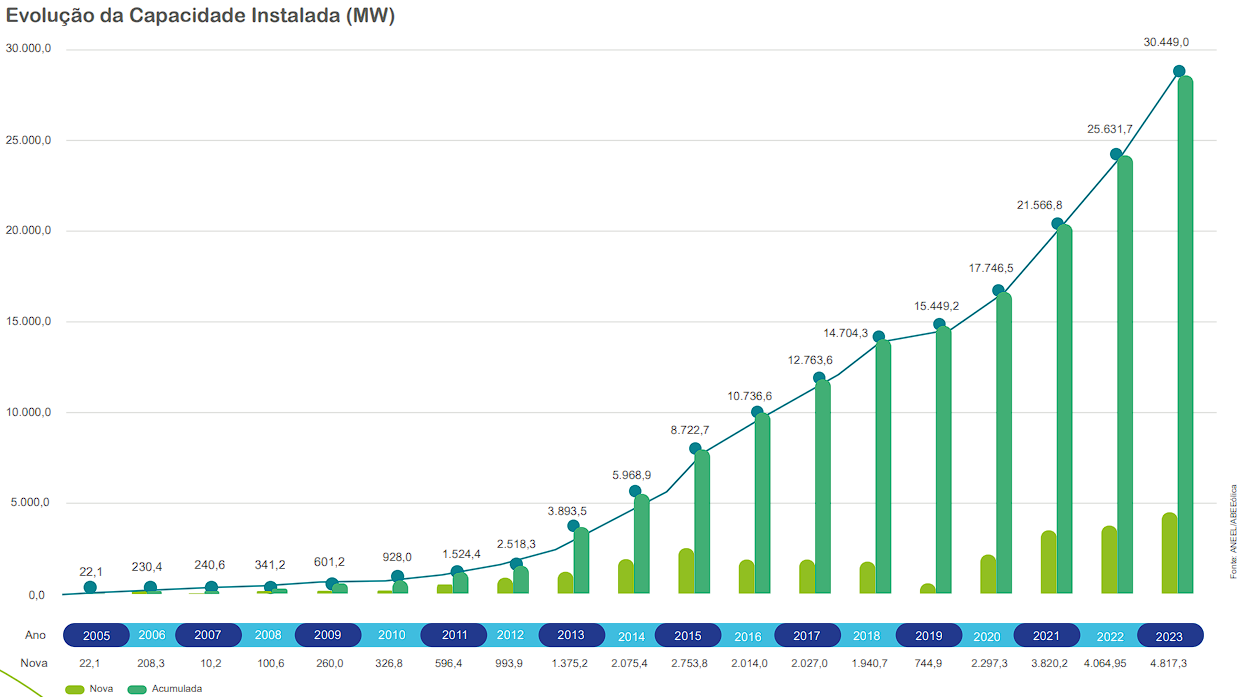
\includegraphics[width=0.8\textwidth]{Figuras/Teorico/evolução da capacidade instalada.png}
    \fonte{\citeonline{abeeolica2024}}
\end{figure}

\par As regiões Nordeste e Sul do Brasil são as que mais se destacam em termos de potencial eólico e número de parques eólicos instalados. O Rio Grande do Norte, a Bahia e o Ceará são os estados líderes na produção de energia eólica no país.

\subsection{Mapeamento do Potencial Eólico}

\par O mapeamento do potencial eólico no Brasil tem sido objeto de diversas pesquisas e estudos ao longo dos anos, realizados por instituições acadêmicas, governamentais e privadas. Esses estudos são fundamentais para identificar as regiões com maior capacidade para a geração de energia eólica e para orientar investimentos no setor. Um exemplo é o Centro de Referência para Energia Solar e Eólica Sérgio de Salvo Brito (CRESESB) com Atlas do Potencial Eólico Brasileiro, representado na Figura \ref{fig:Atlas}.

\begin{figure}[H]
    \caption{Atlas do Potencial Eólico Brasileiro desenvolvido pelo modelo Brams em médias anuais.}      
    \centering
    \label{fig:Atlas}
     \subfigure[Velocidade média anual para a altura de 30 metros.]{
    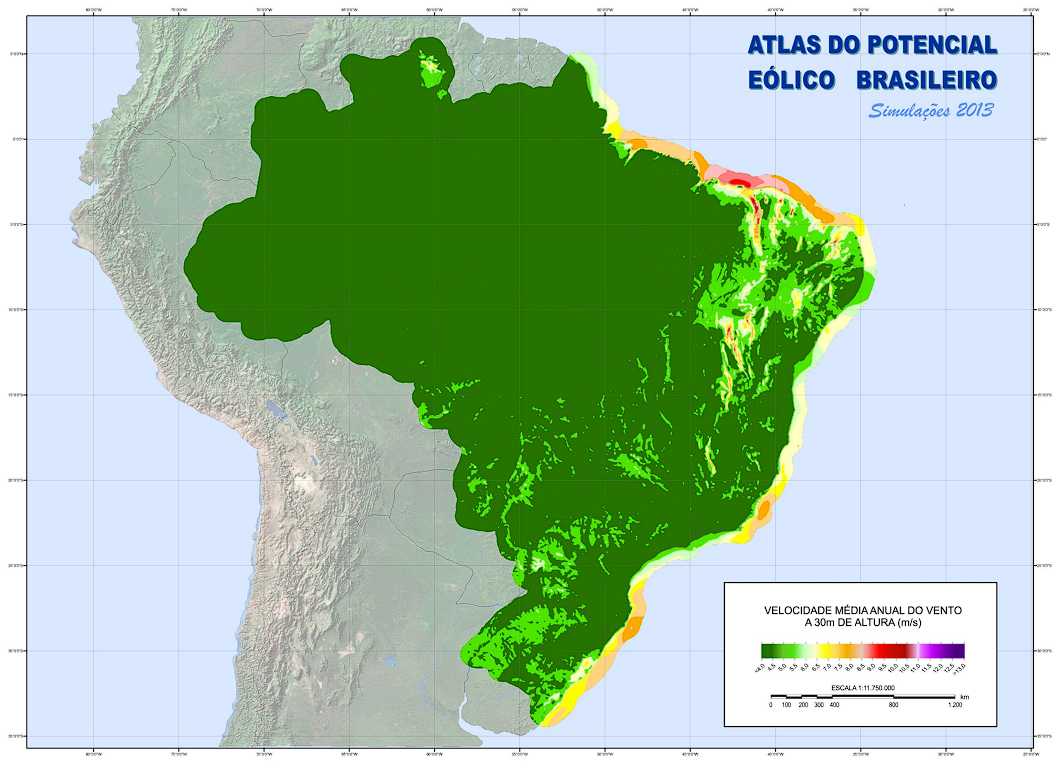
\includegraphics[width=0.45\textwidth]{Figuras/Teorico/Atlas_30m.png}
    \label{fig:Atlas_30m}
    }   
    \hspace{0.05\textwidth}
    \subfigure[Velocidade média anual para a altura de 50 metros.]{
    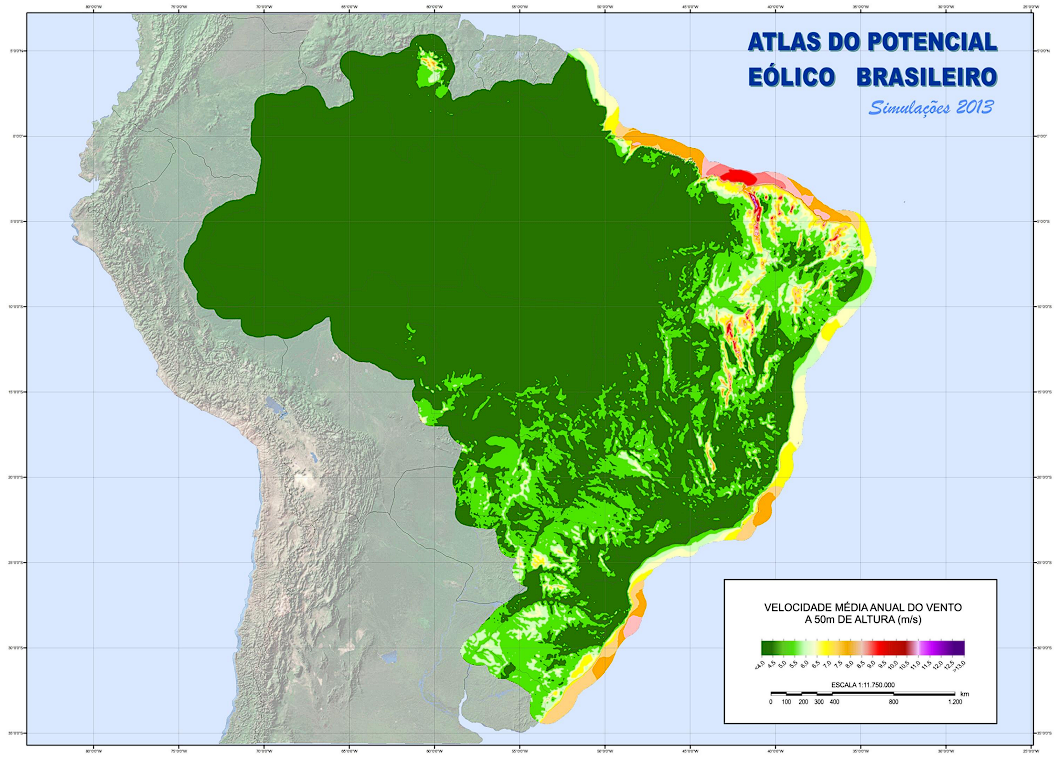
\includegraphics[width=0.45\textwidth]{Figuras/Teorico/Atlas_50m.png}
    \label{fig:Atlas_50m}
    }
    \fonte{\citeonline{cresesb2013}}
    
\end{figure}

\subsection{Cachoeira do Sul}
\par Cachoeira do Sul, localizada no estado do Rio Grande do Sul, é uma cidade que destaca um significativo potencial eólico. A região Sul do Brasil, especialmente o Rio Grande do Sul, possui condições climáticas favoráveis que tornam a energia eólica uma alternativa viável e promissora, como visto na Figura \ref{fig:Atlas_RS}. Assim, a análise das características eólicas de Cachoeira do Sul torna-se um cenário de interesse, não apenas por ser a cidade onde o trabalho está sendo desenvolvido, mas também pela oportunidade de explorar e modelar os recursos eólicos disponíveis.

\begin{figure}[H]
    \caption{Atlas Eólico para o Rio Grande do Sul à altura de 100 metros.}
    \label{fig:Atlas_RS}
    \centering
    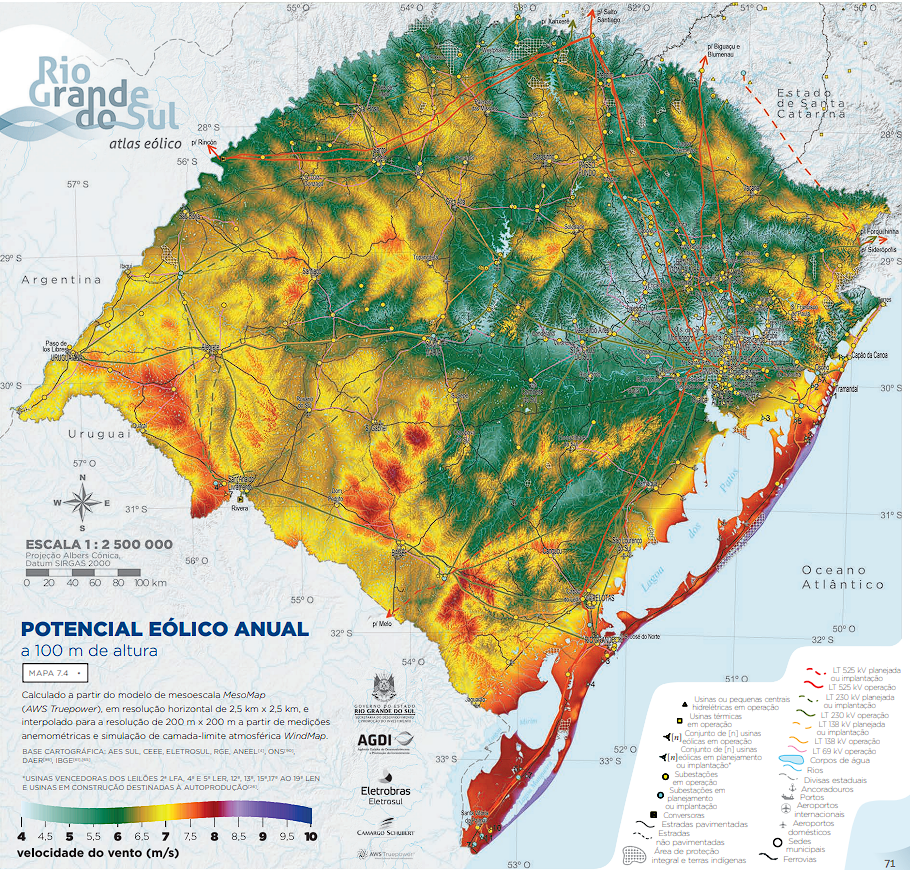
\includegraphics[width=0.8\textwidth]{Figuras/Teorico/Atlas RS.png}
    \fonte{\citeonline{abeeolica2017}}
\end{figure}

\par A velocidade média de vento em Cachoeira do Sul é acima de $2,3\frac{m}{s}$ a uma altura de 10 metros acima do solo, apresentando poucas variações sazonais, como representado na Figura \ref{fig:VelocidadeEMCachoeiraDoSul}. Esta velocidade de vento, embora moderada, indica um bom potencial para a geração de energia eólica.


\begin{figure}[H]
    \caption{Velocidade Média do Vento em Cachoeira do Sul.}      
    \label{fig:VelocidadeEMCachoeiraDoSul}
    \centering
    \includegraphics[width=0.8\textwidth]{Figuras/Teorico/Velocidade média do vento em Cachoeira do Sul.png}
    \fonte{\citeonline{weatherspark2024}}
\end{figure}

\par Para efeitos de comparação foram obtidos dados de velocidade do vento na UFSM de Cachoeira do Sul, através de anemômetro já instalado, visto na Figura \ref{fig:AnemometroCS}. Os dados de velocidade foram obtidos para o ano de 2023 com intervalo de uma hora a uma altura de aproximadamente três metros, gerando no gráfico da Figura \ref{fig:DadosAnemometroCS}. Para efeitos de analise, os dados obtidos foram inseridos na distribuição de Weibull visto na Figura \ref{fig:DistribuicaoWeibull}. 

\begin{figure}[H]
    \caption{Fotografia do Anemômetro instalado na UFSM Campus Cachoeira do Sul.}      
    \label{fig:AnemometroCS}
    \centering
    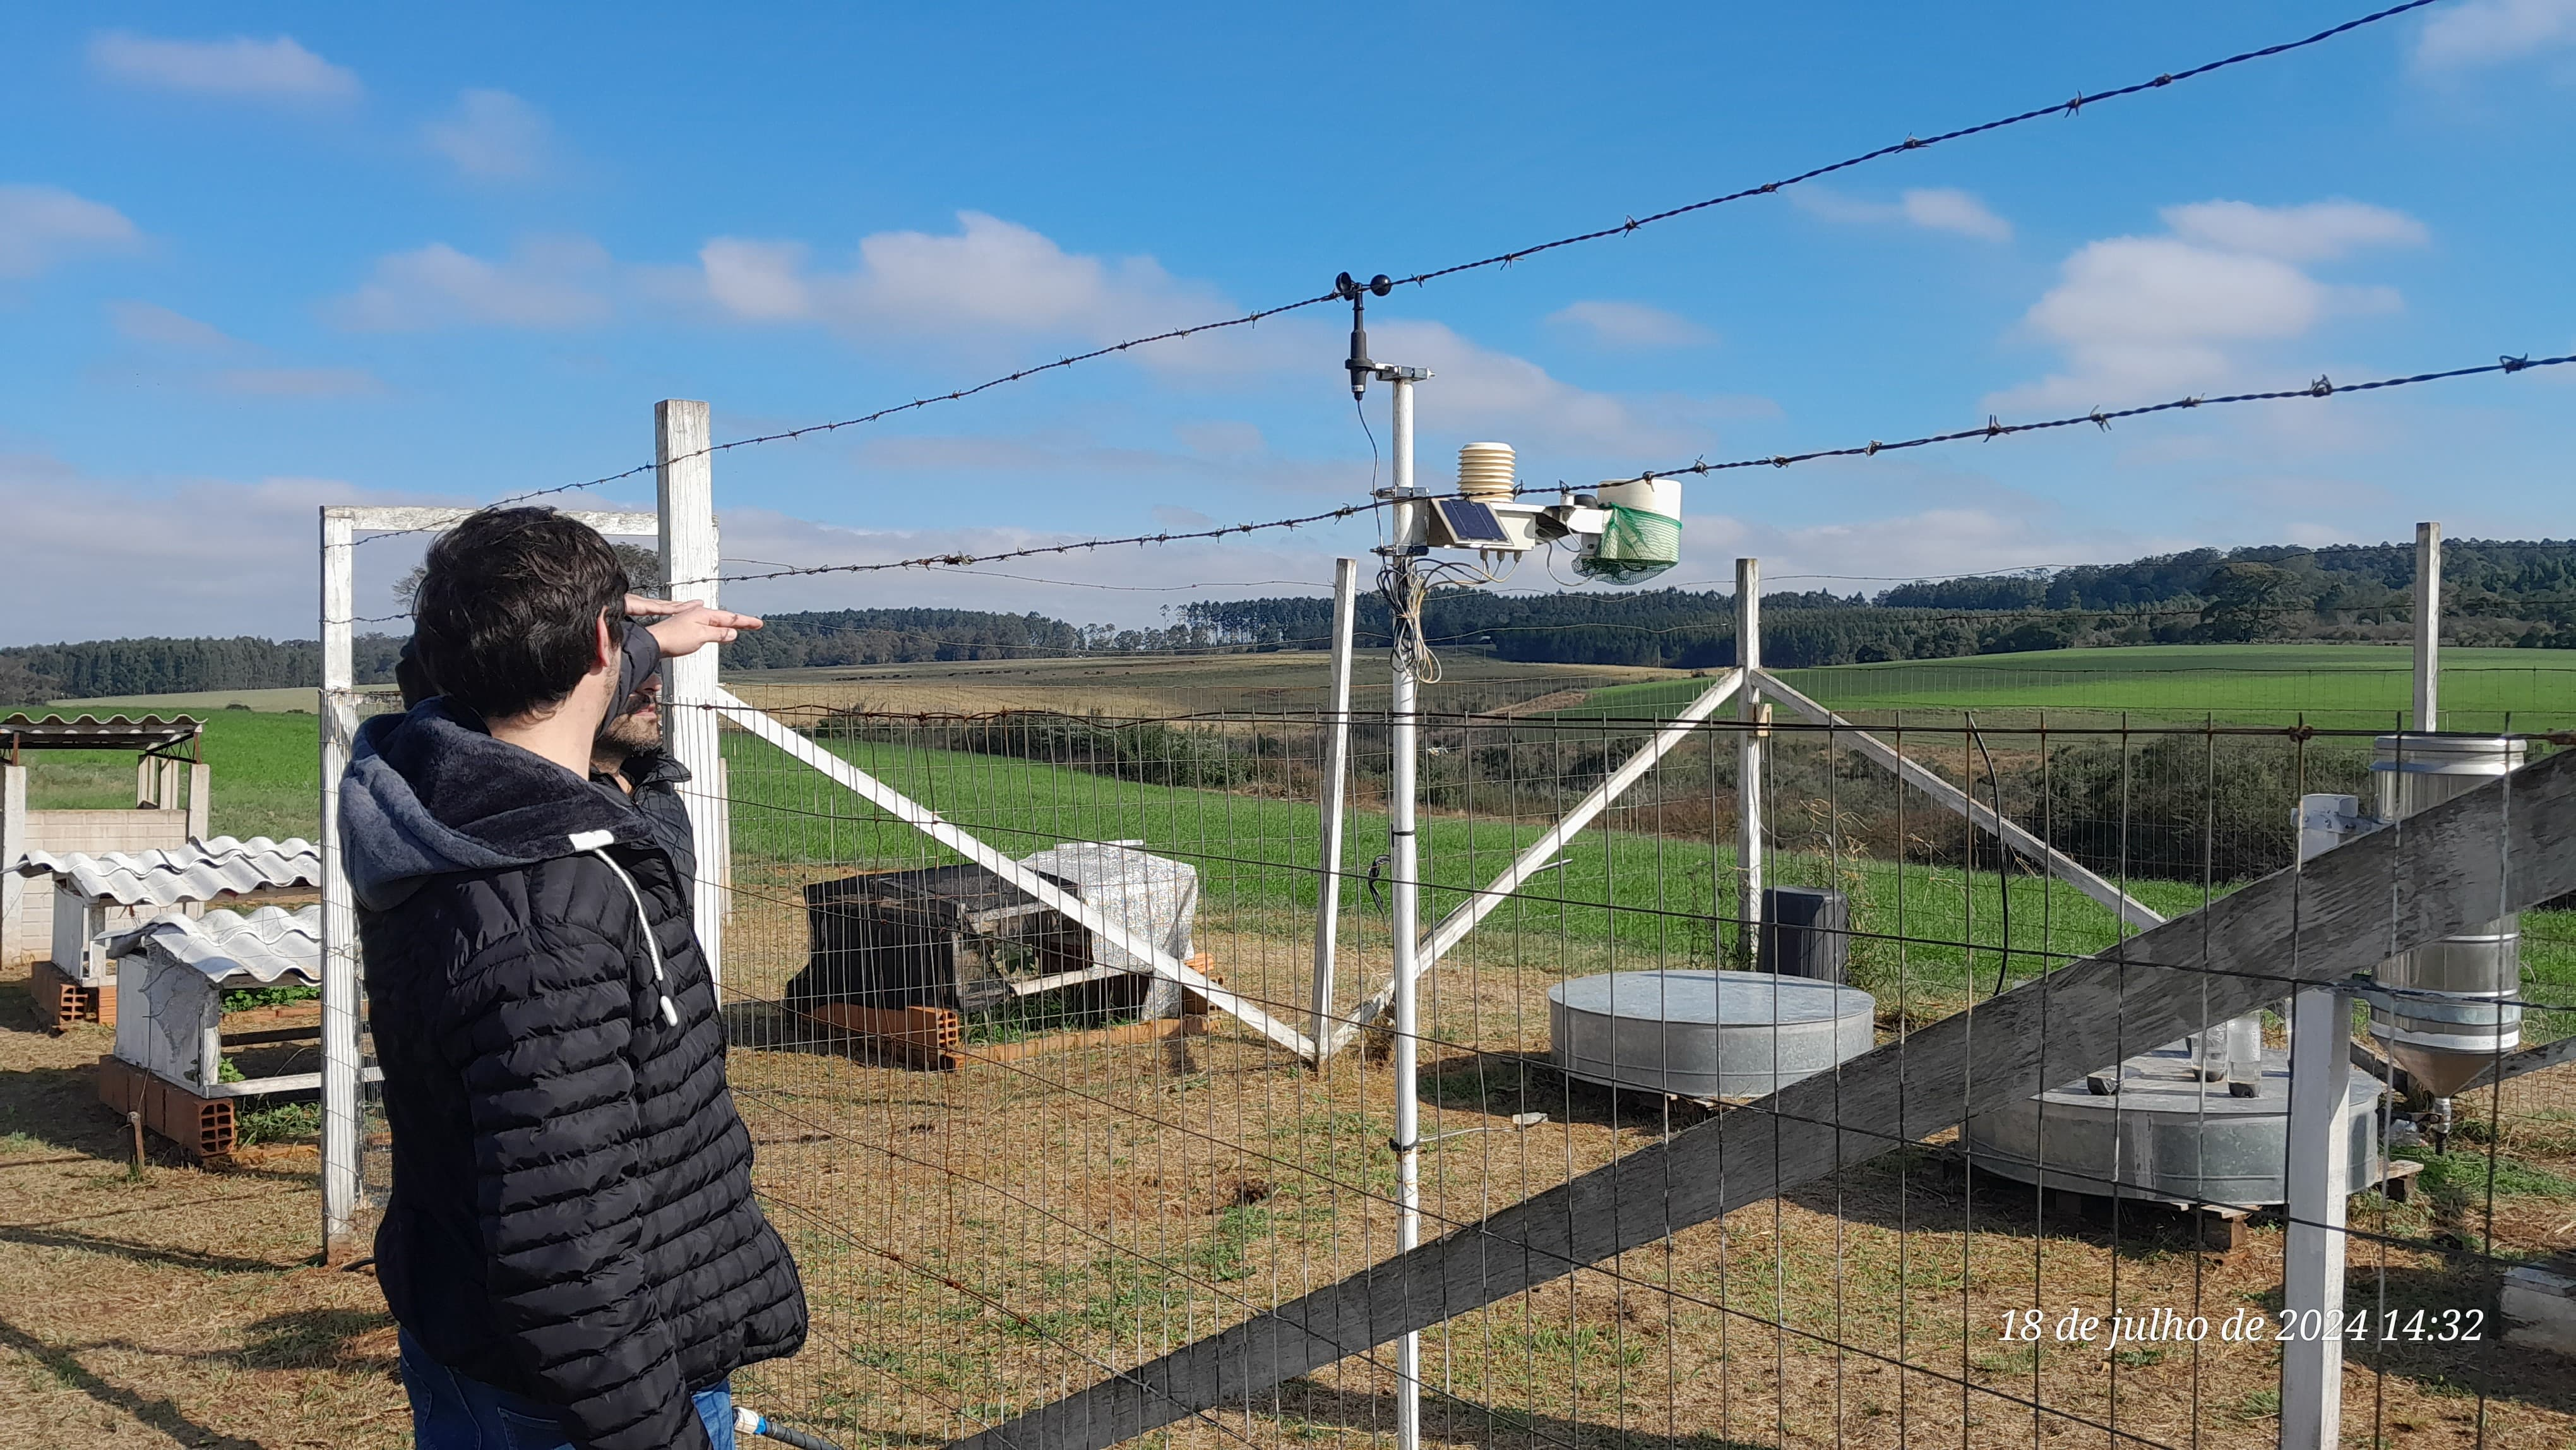
\includegraphics[width=0.8\textwidth]{Figuras/Teorico/anemometro_CampusUFSM.jpg}    
\end{figure}

\begin{figure}[H]
    \caption{Gráfico dos dados do Anemômetro instalado na UFSM Campus Cachoeira do Sul.}      
    \label{fig:DadosAnemometroCS}
    \centering
    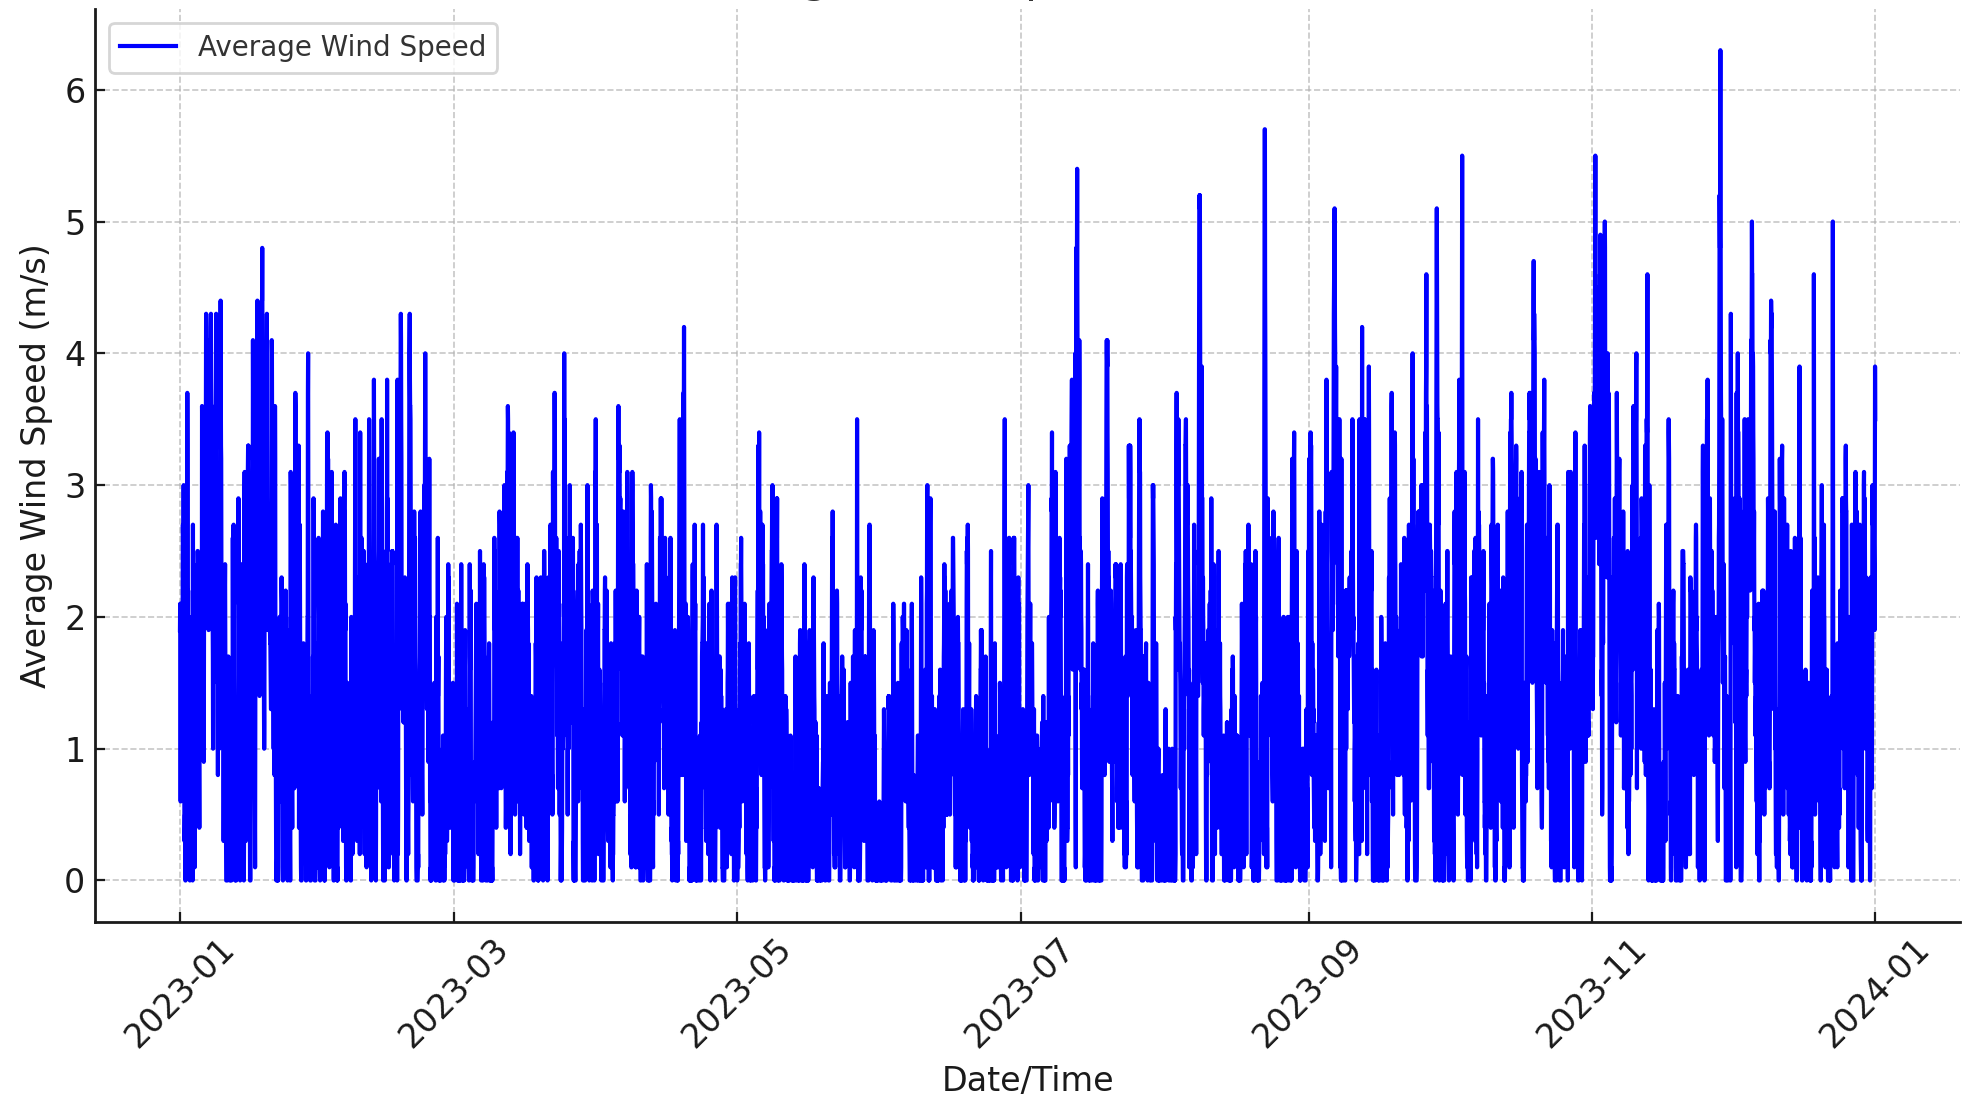
\includegraphics[width=0.8\textwidth]{Figuras/Teorico/Average Wind Speed Over Time2.png}    
\end{figure}

\begin{figure}[H]
    \caption{Distribuição de Weibull dos dados do Anemômetro instalado na UFSM Campus Cachoeira do Sul.}      
    \label{fig:DistribuicaoWeibull}
    \centering
    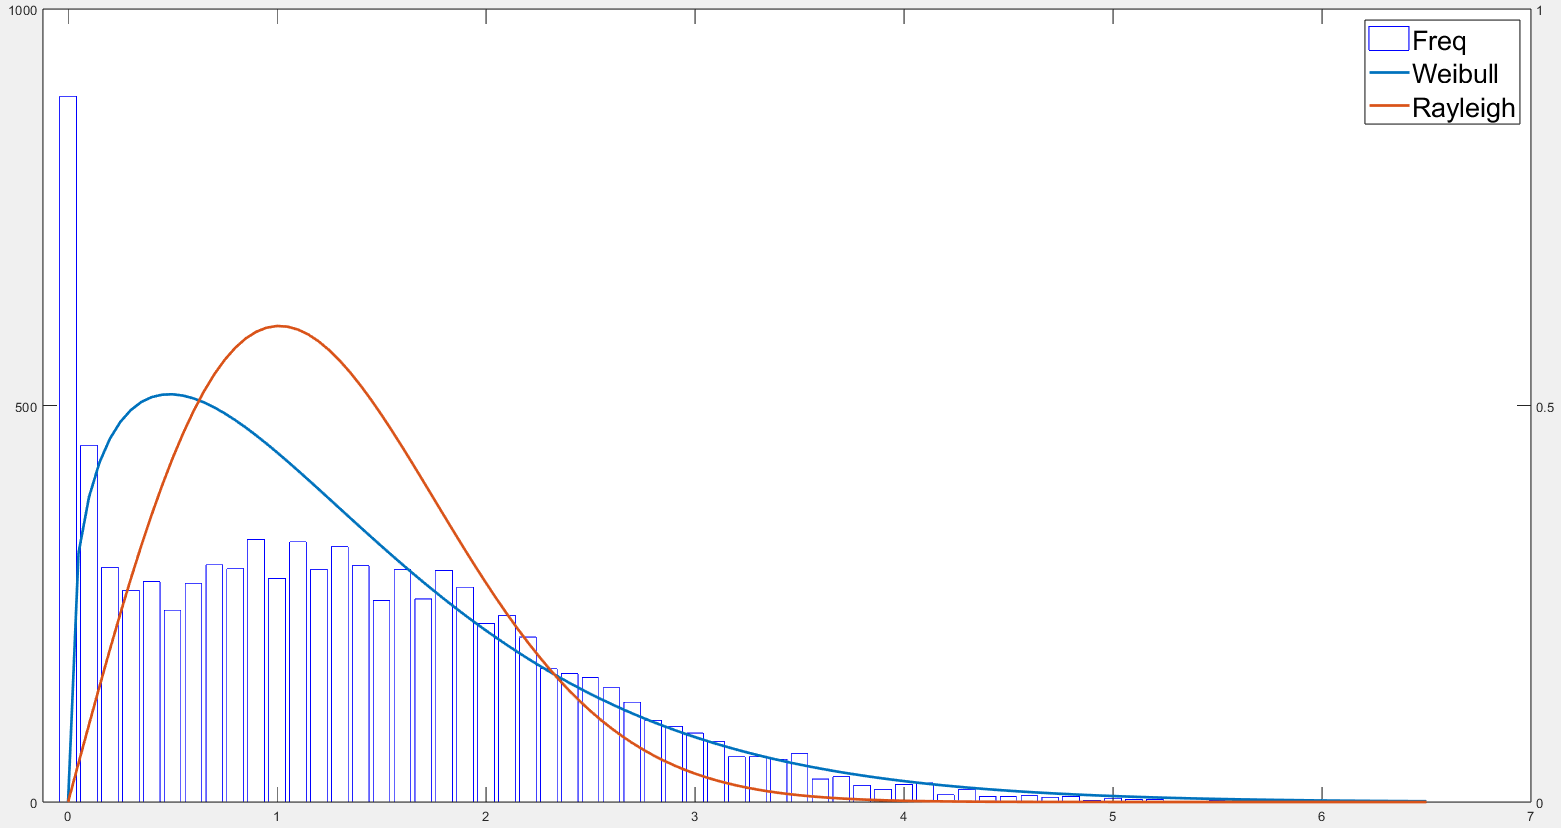
\includegraphics[width=0.8\textwidth]{Figuras/Teorico/DistribuicaoWeibull.png}    
\end{figure}


\par Devido ao anemômetro estar muito próximo ao solo, os valores obtidos apresentam muitas variações. Conforme recomendado por \citeonline{fadigas2011}, o ideal é que o anemômetro esteja posicionado à altura do cubo do aerogerador. Esta altura permite uma medição mais precisa e representativa das condições de vento que a turbina eólica se encontrará, minimizando as interferências causadas pela rugosidade do solo e por obstáculos próximos, resultando em dados mais confiáveis para a modelagem do vento e a operação eficiente dos aerogeradores.


\section{Analise dos Ventos}

\par
    
\begin{figure}[H]
    \caption{Camadas da Atmosfera}
    \label{fig:atmosfera}
    \centering
    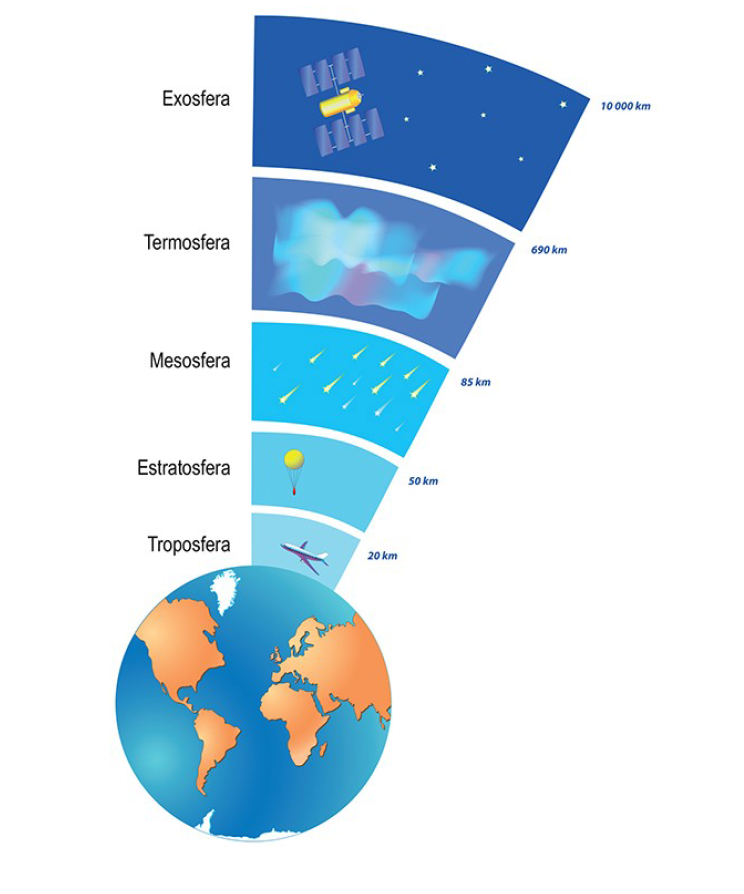
\includegraphics[width=0.5\textwidth]{Figuras/Teorico/atmo.png}
    \fonte{\citeonline{site:Atmosfera}}
\end{figure}

\par Entendendo que os principais fenômenos envolvendo vento está relacionado a troposfera, também é essencial entender que o ar se comporta como um fluido, que em movimento é percebido como vento. Assim como qualquer fluido, o ar está sujeito a influências físicas como variações térmicas e variação de pressão. Um bom exemplo está na radiação solar, que provoca variações de temperatura no ar, criando áreas de alta e baixa pressão que, por sua vez, geram movimento de ar das áreas de alta pressão para as de baixa pressão, resultando na formação de ventos.

\par Além dos efeitos térmicos, a topografia do terreno desempenha um papel crucial na modelagem e comportamento dos ventos. Montanhas, vales, florestas e corpos d'água modificam significativamente a direção e a velocidade dos ventos, gerando padrões complexos que precisam ser cuidadosamente estudados para a instalação eficiente de aerogeradores.

\par De acordo com \citeonline{fadigas2011}, no passado os dados sobre recursos eólicos eram avaliados exclusivamente com base em critérios meteorológicos, considerando apenas o movimento das grandes massas de ar, tornando as informações insuficientes e inadequadas. Por exemplo, as torres meteorológicas não esclareciam as condições do vento em terrenos específicos nem a variação da velocidade do vento com a altura.

\par Nas últimas décadas, conforme destacado por \citeonline{fadigas2011}, campanhas de medição de ventos começaram a ser realizadas em vários países. O objetivo dessas campanhas é obter uma avaliação mais precisa das condições do vento em diferentes tipos de relevo, rugosidade do solo e alturas variadas, visando ao aproveitamento energético otimizado dos ventos. Atualmente, existem bases de dados e mapas eólicos com informações detalhadas coletadas ao longo de vários anos. Esses dados são provenientes tanto de torres anemométricas quanto de medições realizadas nas próprias centrais eólicas.

\par Entretanto, mesmo com a disponibilidade de mapas ou atlas eólicos, é fundamental realizar medições locais específicas para determinar o potencial eólico com precisão. Recomenda-se a instalação de torres anemométricas adaptadas ao terreno e à rugosidade local, preferencialmente posicionadas à altura do cubo do aerogerador. Abrangendo um período mínimo de um ano, para capturar a variabilidade sazonal e mensal dos ventos, garantindo uma avaliação completa do potencial eólico da região.

 \subsection{Circulação dos Ventos}
 \par Os ventos podem ser classificados de acordo com a  circulação global ou local. Os de circulação global resultam da incidência solar desigual no planeta, variando conforme a distribuição geográfica, o período do dia e a distribuição anual \cite{martins2008}.Já os ventos de circulação local são influenciados por características específicas de uma região, como a topografia, a presença de corpos d'água e as diferenças de temperatura entre áreas adjacentes.
 
 \par A radiação solar absorvida de maneira desigual pela Terra é mais intensa próximo a linha do Equador, gerando desequilíbrio em relação aos polos. Buscando o equilíbrio térmico, as massas de ar quente e úmida presente na região dos trópicos movimentam-se para os polos, enquanto as massas de ar fria e seca deslocam-se em sentido a linha do Equador, fechando o ciclo, conforme visto na figura \ref{fig:FormacaoDosVentos}.

\begin{figure}[H]
    \caption{Formação dos ventos devido ao movimento das massas de ar}
    \label{fig:FormacaoDosVentos}
    \centering
    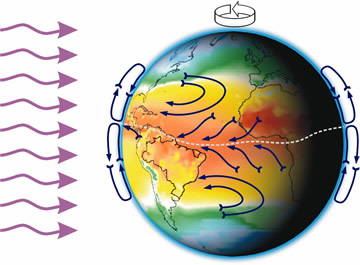
\includegraphics[width=0.5\textwidth]{Figuras/Teorico/FormacaoDosVentos.png}
    \fonte{\citeonline{cepel2001}}
\end{figure}

\par A rotação da Terra também influencia a formação dos ventos, criando padrões distintos: no Hemisfério Norte e no Hemisfério Sul. De acordo com \citeonline{reboita2012} e \citeonline{pinto2014}, devido à força de Coriolis, no Hemisfério Sul, o vento movimenta-se em direção do polo para o equador sofrendo um deslocamento de sentido negativo ao eixo X. Ao modo que o vento indo em direção ao polo oriundo do equador sofre um desvio positivo em relação ao eixo X, como visto na figura \ref{fig:circulação geral da atmosfera terrestre}. 

\begin{figure}[H]
    \caption{Esquema representativo da circulação geral da atmosfera terrestre.}
    \label{fig:circulação geral da atmosfera terrestre}
    \centering
    \includegraphics[width=0.5\textwidth]{Figuras/Teorico/Regiões de Circulacao.png}
    \fonte{Retirado \cite{rocha2023} baseado em \cite{reboita2012}}
\end{figure}

\par Devido à inclinação do eixo de rotação da Terra em relação ao plano de sua órbita ao redor do Sol, há variações sazonais na intensidade e direção do vento em qualquer lugar do planeta. Além do gradiente de pressão e da força de Coriolis (causada pela rotação da Terra), os ventos atmosféricos também são afetados por forças gravitacionais, inércia do ar e fricção com a superfície terrestre, resultando em turbulência.

% \par A Figura \ref{fig:FormacaoDosVentos} ilustra o comportamento dos ventos de circulação global que cobrem todo o planeta.

\par Nas grandes altitudes, o ar se movimenta seguindo linhas de igual pressão, chamadas isolinhas. Esse movimento de massas de ar a mais de 600 metros de altitude é conhecido como ventos geotrópicos. Nessa altura, o fluxo de ar não é influenciado pela superfície terrestre. Em altitudes mais baixas, as diferentes superfícies da Terra, como oceanos, terras e vegetação, afetam significativamente o fluxo de ar devido a variações de pressão, diferentes níveis de absorção da radiação solar e umidade, influenciando o clima próximo à superfície. Esta região da atmosfera, onde os ventos são afetados pela superfície, é chamada de camada limite.

\par Além de movimentos em escala global (Equador - polos), também há formação de ventos em escala local, como "mar para o continente", "vales para as montanhas" e vice-versa.

\par As brisas marítimas e terrestres ocorrem em áreas costeiras devido às diferentes capacidades de absorção de calor da terra e do mar. Durante o dia, a terra aquece mais rapidamente que o mar, elevando a temperatura do ar sobre a terra e criando uma corrente de ar que sopra do mar para a terra, conhecida como brisa marítima. À noite, a terra esfria mais rapidamente que a água, resultando em uma corrente de ar que sopra da terra para o mar, chamada de brisa terrestre, conforme demonstra a figura \ref{fig:brisaTerrestreMaritima}.

\begin{figure}[H]
    \caption{Circulação de ventos em escala local.(a) Brisa Marítima e (b) Brisa Terrestre. }
    \label{fig:brisaTerrestreMaritima}
    \centering
    \includegraphics[width=0.7\textwidth]{Figuras/Teorico/brisaMaritima_brisaTerrestre.png}
    \fonte{Adaptado da \citeonline{aneel2009}}
\end{figure}

\par Os ventos em regiões montanhosas e vales também seguem um padrão diário. Durante o dia, o ar frio nas montanhas se aquece e sobe, permitindo que o ar mais frio dos vales flua para substituir o ar quente que subiu. À noite, o processo se inverte: o ar frio das montanhas desce para os vales, enquanto o ar quente dos vales sobe em direção às montanhas, como ilustra a figura \ref{fig:brisaValeMotanha}. 

\begin{figure}[H]
    \caption{Circulação de ventos em escala local.(a) Brisa do Vale e (b) Brisa da Montanha. }
    \label{fig:brisaValeMotanha}
    \centering
    \includegraphics[width=0.7\textwidth]{Figuras/Teorico/Brisa do Vale e da Montanha.png}
    \fonte{Adaptado da \citeonline{aneel2009}}
\end{figure}

 \subsection{Classificação dos Movimentos Atmosféricos}
\par A formação dos ventos descrita anteriormente é apenas um exemplo dos muitos processos que ocorrem na superfície da Terra, muitos dos quais são influenciados por variações climáticas em diferentes escalas de tempo e espaço. Na meteorologia, há uma classificação específica para esses movimentos atmosféricos.
\par Utilizando a classificação de Lutgens e Tarbuck, descrito em \cite{lutgens2012atmosphere} e exemplificado em \cite{pinto2014}, existem três grandes escalas de comprimento na meteorologia: microescala, mesoescala e macroescala. Esta última é subdividida em duas: escala sinóptica e escala planetária (ou global), como destaca a tabela \ref{tab:escalar-atmosféricas}.

\begin{table}[h]
\caption{Principais características das escalas atmosféricas}
\centering
\begin{tabularx}{\textwidth}{X|X|X|X}
\hline
\textbf{Escala} & \textbf{Tamanho} & \textbf{Duração} & \textbf{Fenômeno} \\
\hline
Microescala & Menos que 1 km & Segundos a minutos
 & Semanas a anos \\
\hline
Mesoescala & 1 a 100 km & Minutos a dias & tempestades, tornados e brisa terrestre \\
\hline
Macroescala - Sinóptica & 100 a 5000 km & Dias a semanas
 & Ciclones de latitudes médias, anticiclones e furacões \\
\hline
Macroescala - Planetária & 1000 a 40.000 km & Semanas a anos & Ventos alísios e ventos do oeste \\
\hline
\end{tabularx}

\label{tab:escalar-atmosféricas}
\end{table}

\par Os movimentos atmosféricos variam significativamente no tempo e no espaço, abrangendo intervalos que vão de segundos a meses e distâncias que variam de centímetros a milhares de quilômetros. As variações na velocidade do vento ao longo do tempo podem ser classificadas, de acordo com \cite{pinto2014}, em várias categorias:


\begin{itemize}
\item[a)] \textbf{Interanuais}
    \begin{itemize}
        \item \textbf{Período:} Ocorrem em períodos superiores a um ano.
        \item \textbf{Impacto:} Podem ter um impacto significativo na produção de energia em turbinas eólicas de grande porte.
        \item \textbf{Dados Necessários:}
        \begin{itemize}
            \item Mínimo de 30 anos de dados para determinar valores climáticos de longo prazo.
            \item Pelo menos 5 anos de dados para estabelecer uma média anual confiável de velocidade do vento para uma região específica.
        \end{itemize}
    \end{itemize}

    \item[b)] \textbf{Anuais}
    \begin{itemize}
        \item \textbf{Período:} Ocorrências devido a variações relevantes na média mensal ou sazonal da velocidade do vento.
    \end{itemize}

    \item[c)] \textbf{Diurnas}
    \begin{itemize}
        \item \textbf{Localização:} Ocorrem em latitudes temperadas e tropicais.
        \item \textbf{Período:} Variam significativamente na escala diária.
        \item \textbf{Causa:} Devidas às diferenças de aquecimento na superfície terrestre durante o ciclo diário de radiação solar.
        \item \textbf{Exemplo:}
        \begin{itemize}
            \item Aumento da velocidade do vento durante o dia.
            \item Diminuição da velocidade do vento durante as horas noturnas, da meia-noite ao amanhecer.
        \end{itemize}
    \end{itemize}

    \item[d)] \textbf{De Curto Prazo}
    \begin{itemize}
        \item \textbf{Período:} Geralmente ocorrem em períodos de 10 minutos ou menos.
        \item \textbf{Exemplos:} Rajadas de vento e turbulências.
        \item \textbf{Turbulências:}
        \begin{itemize}
            \item \textbf{Definição:} Flutuações aleatórias na velocidade do vento que afetam a média geral.
            \item \textbf{Direções:}
            \begin{itemize}
                \item Longitudinal (ao longo da direção do vento).
                \item Lateral (perpendicular ao vento).
                \item Vertical.
            \end{itemize}
        \end{itemize}
        \item \textbf{Rajadas:}
        \begin{itemize}
            \item \textbf{Definição:} Evento discreto dentro de um campo turbulento de vento.
            \item \textbf{Caracterização:} Medição de quatro fatores principais:
            \begin{itemize}
                \item Amplitude.
                \item Duração.
                \item Variação máxima da rajada.
                \item Tempo de resposta.
            \end{itemize}
        \end{itemize}
        \item \textbf{Impacto nas Turbinas Eólicas:} Flutuações turbulentas na velocidade induzem forças cíclicas na estrutura da turbina, causando problemas de estresse e fadiga. Além de que, influenciam diretamente na operação, controle da turbina eólica e na qualidade da potência gerada. A figura \ref{fig:velocidade ao longo do tempo}\subref{fig:CurtaDuracao} demostra uma variação típica de curta duração. 
    \end{itemize}
\end{itemize}

\begin{figure}[H]
    \caption{Variações de velocidade ao longo do tempo na Dinamarca.}      
    \centering
    \label{fig:velocidade ao longo do tempo}
     \subfigure[Variações de velocidade do vento Diurno, intervalo de três horas.]{
    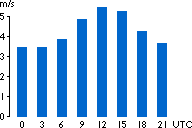
\includegraphics[width=0.45\textwidth]{Figuras/Teorico/diurnal.png}
    \label{fig:diurno}
    }   
    \hspace{0.05\textwidth}
    \subfigure[Variações de velocidade do vento em curta duração.]{
    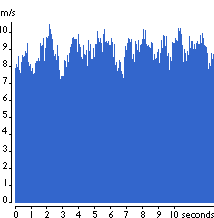
\includegraphics[width=0.45\textwidth]{Figuras/Teorico/turbulencia10s.png}
    \label{fig:CurtaDuracao}
    }
    \fonte{\citeonline{danishwind2024}}
    
\end{figure}

 \subsection{Forças Fundamentais que Regem o Movimento do Vento}
 \par O vento é definido como o movimento das massas de ar na atmosfera. Este fenômeno pode ser analisado como uma interação dinâmica entre várias parcelas de ar em movimento contínuo. Esse movimento resulta da interação de diversas forças que se intensificam ou se atenuam mutuamente. As principais forças envolvidas são cinco:

 \begin{itemize}
    \item[a)] \textbf{Força do Gradiente de Pressão}
    \begin{itemize}
        \item \textbf{Descrição:} A força do gradiente de pressão é responsável por mover o ar das áreas de alta pressão para as áreas de baixa pressão. Este fenômeno é ocasionado pelo aquecimento desigual da superfície terrestre devido à radiação solar, criando zonas distintas de alta e baixa pressão. O desequilíbrio resultante impulsiona o movimento do vento, que naturalmente se desloca da região de maior para a de menor pressão.
%      \item \textbf{Fórmula:} 
%          \begin{equation}
%              \vec{\nabla}_p = \frac{\partial p}{\partial x} \vec{i} + \frac{\partial p}{\partial y} \vec{j} + \frac{\partial p}{\partial z} \vec{k}
%          \end{equation}
%          \begin{equation}
%              \vec{\nabla}_p = \rho \vec{g}
%          \end{equation}
%          \begin{equation}
%              \mathbf{F}_{gpx} = -\vec{\nabla}_p
%              \label{eq:force_pressure_gradient}
%              \caption{Força é o gradiente negativo de pressão.}
%          \end{equation}
        \item \textbf{Importância:} Esta força é fundamental na formação de ventos e sistemas meteorológicos.
    \end{itemize}
    
    \item[b)] \textbf{Força de Coriolis}
    \begin{itemize}
        \item \textbf{Descrição:} A força de Coriolis, ou também efeito de Coriolis, nomeada em homenagem ao matemático e engenheiro Gaspard Gustabe de Coriolis. É uma força inercial que é resultante da rotação da Terra, que causa movimentos circulares ou em espiral entre os polos e o equador. Seu efeito é percebido na deflexão dos ventos: para a direita no hemisfério norte e para a esquerda no hemisfério sul.
        \item \textbf{Fórmula:} Para efeito de estudo em energia eólica, de acordo com \citeonline{pinto2014}, a formula da força de Coriolis é dada por:
            \begin{equation}
                F_{co} = 2\Omega V \sin{\Phi},
                \label{eq:placeholder_label}
                %\caption{Expressão para a força de Coriolis.}
            \end{equation}
            em que:
            \begin{align*}
                F_{co} & \text{ é a força de Coriolis,} \\
                \Omega & \text{ é a velocidade angular da Terra \( (7.29 \times 10^{-5} \, \text{rad/s}) \),} \\
                V & \text{ é a velocidade da partícula \( (\text{m/s}) \),} \\
                \Phi & \text{ é a latitude da partícula em graus \( (\text{em graus}) \).}
            \end{align*}
        \item \textbf{Importância:} Esta força é crucial na formação de correntes de vento de grande escala e fenômenos climáticos como ciclones.
    \end{itemize}
    
    \item[c)] \textbf{Força Centrífuga}
    \begin{itemize}
        \item \textbf{Descrição:} A força centrífuga é uma força aparente que atua sobre um corpo em rotação, afastando-o do centro de rotação.
        \item \textbf{Fórmula:} 
            \begin{equation}
                F = m \omega^2 r
                \label{eq:placeholder}
                %\caption{Força Centrífuga}
            \end{equation}
        \item \textbf{Importância:} Esta força é relevante em sistemas de referência rotativos e afeta o movimento de massas de ar em sistemas de baixa pressão.
    \end{itemize}
    
    \item[d)] \textbf{Força de Atrito}
    \begin{itemize}
        \item \textbf{Descrição:} A força de atrito é a força que resiste ao movimento relativo de superfícies ou camadas de ar em contato.       
        \item \textbf{Importância:} Esta força reduz a velocidade dos ventos próximos à superfície da Terra e influencia a formação de padrões climáticos locais.
    \end{itemize}
    
    \item[e)] \textbf{Força da Gravidade}
    \begin{itemize}
        \item \textbf{Descrição:} A força da gravidade é a força que atrai os objetos em direção ao centro da Terra.         
        \item \textbf{Importância:} A gravidade é fundamental na manutenção da atmosfera terrestre e afeta o movimento vertical do ar.
    \end{itemize}
\end{itemize}


    \section{Perfil de Vento}
    
        \par Conforme demonstrado por estudos em mecânica dos fluidos, a velocidade de um fluido que flui próximo a uma superfície é reduzida a zero devido ao atrito entre o fluido e a superfície. Ao observar o perfil de velocidade do fluido em relação à altura, percebe-se que a velocidade aumenta de zero até alcançar a velocidade de escoamento ($\nu$). Essa variação é mais acentuada próxima à superfície e diminui em altitudes mais elevadas \cite{batchelor2000}. 

        \par A região próxima à superfície, onde essa mudança rápida de velocidade ocorre, é denominada camada limite, como ilustrado na Figura \ref{fig:Esquema do perfil de velocidades}\subref{fig:velocidades superficie plana}. Dentro dessa camada, o ar geralmente apresenta turbulência, influenciada por fatores como densidade e viscosidade do fluido, rugosidade da superfície e a presença de obstáculos \cite{schlichting2000}.

        \begin{figure}[H]
            \caption{Esquema do perfil de velocidades sobre uma superfície plana. }
            \label{fig:Esquema do perfil de velocidades}
            \centering
             \subfigure[Alto efeito viscoso. (b) Baixo efeito viscoso.]{
                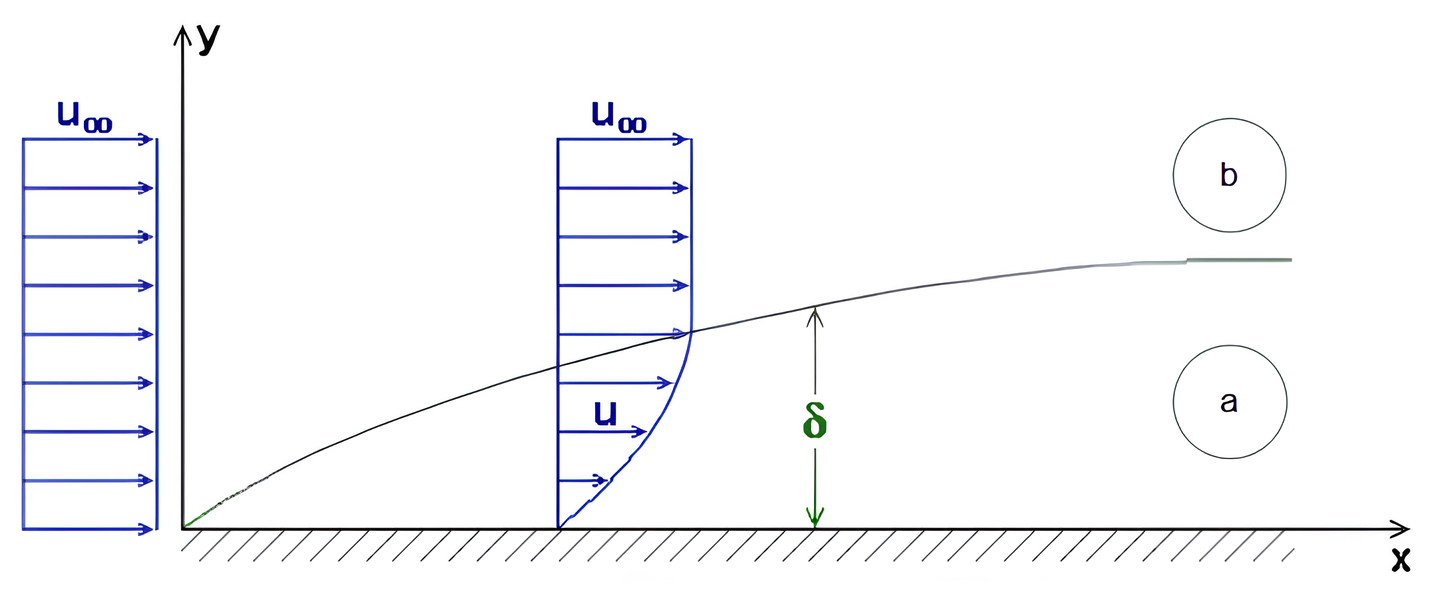
\includegraphics[width=0.7\textwidth]{Figuras/Teorico/velocidades sobre uma placa plana.png}
                \label{fig:velocidades superficie plana}
                }              
            \fonte{\citeonline{camada_limite}}
        \end{figure}

        \par A potência contida no vento é função da densidade do ar, que, por sua vez, é influenciada pela temperatura e pressão, ambas variáveis com a altura em relação ao solo. Como os aerogeradores em operação comercial são instalados dentro da camada limite (até 150 m), é crucial compreender a distribuição da velocidade do vento com a altura. Isso é importante porque a velocidade do vento determina a produtividade de uma turbina instalada em uma torre de certa altura e influencia a vida útil das pás do rotor, que são submetidas a cargas cíclicas devido à turbulência do vento.

        \par Os ventos turbulentos resultam da dissipação da energia cinética em energia térmica através da criação e destruição de pequenas rajadas progressivas. Esses ventos são caracterizados por várias propriedades estatísticas: intensidade, função densidade de probabilidade, autocorrelação, escala integral de tempo e função densidade espectral de potência. Detalhados com mais detalhes por \citeonline{rohatgi1994wind}, apud \citeonline{manwell2004wind}.

        \par Em estudos sobre o aproveitamento energético dos ventos, dois modelos matemáticos são comumente utilizados para representar o perfil vertical dos ventos: a lei da potência e a lei logarítmica \cite{fadigas2011}.

        \par A lei da potência é um modelo simples derivado de estudos sobre a camada limite em uma placa plana. É fácil de aplicar, mas não oferece alta precisão. A lei da potência é expressa pela seguinte fórmula:

        \begin{equation}
            V = V_r \left( \frac{H}{H_r} \right)^n
            \label{eq:lei da potência}
        \end{equation}
      em que 
        \begin{itemize}
            \item $V$ = velocidade do vento na altura (H)
            \item $V_r$ = velocidade do vento na altura de referência (medida)
            \item $H$ = altura desejada
            \item $H_r$ = altura de referência
            \item $n$ = expoente da lei de potência
        \end{itemize}

        \par O expoente $n$ representa a influência da natureza do terreno no perfil vertical da velocidade do vento e indica a correspondência entre o perfil do vento e o fluxo sobre uma placa plana. Além da natureza do terreno, o expoente $n$ também é influenciado pela hora do dia, temperatura, parâmetros térmicos e mecânicos, e estação do ano. Em outras palavras, o expoente $n$ não é constante e pode variar conforme as condições ambientais mudam ao longo dos meses. A Tabela \ref{tab:valores de n para tipos de superficie} apresenta alguns valores de $n$ para diferentes tipos de terrenos planos \cite{fadigas2011}.

        \begin{table}[h!]
            \centering
            \caption{Fator $n$ para diferentes tipos de superfícies}
            \label{tab:valores de n para tipos de superficie}
            \begin{tabular}{l|c}
                \hline
                \textbf{DESCRIÇÃO DO TERRENO} & \textbf{FATOR $n$} \\ \hline
                Superfície lisa, lago ou oceano & 0,10 \\ \hline
                Grama baixa & 0,14 \\ \hline
                Vegetação rasteira (até 0,3m), árvores ocasionais & 0,16 \\ \hline
                Arbustos, árvores ocasionais & 0,20 \\ \hline
                Árvores, construções ocasionais & 0,22 -- 0,24 \\ \hline
                Áreas residenciais & 0,28 -- 0,40 \\ \hline
            \end{tabular}
            \fonte{\citeonline{hirata1985} apud \citeonline{dutra2001}}
        \end{table}

        \par É preciso ter cautela ao aplicar a lei da potência em regiões com relevo acidentado, como terrenos montanhosos ou com depressões, e para alturas superiores a 50 metros.

        \par O modelo baseado na lei logarítmica é mais adequado e realista para entender o perfil vertical do vento, pois considera que o fluxo atmosférico é altamente turbulento \cite{troen1989,silva1999,fadigas2011}. Este modelo utiliza o parâmetro "L – comprimento de mistura", que incorpora a constante de Von Kármán $K_c$ e o comprimento de rugosidade $Z_o$, reconhecendo que a superfície da Terra nunca é completamente lisa.

        \par Para altas velocidades, o perfil vertical do vento é descrito pela lei logarítmica:
        \begin{equation}
            V(z) = \frac{v_0}{K_c} \ln \left( \frac{z}{z_0} \right)
        \end{equation}

        em que
        \begin{itemize}
            \item $V(z)$ é a velocidade do vento na altura $z$;
            \item $z_0$ é o comprimento de rugosidade que caracteriza a rugosidade do terreno;
            \item $K_c$ é a constante de Von Kármán ($K_c = 0,4$);
            \item $v_0$ é a velocidade de atrito, relacionada com a tensão de cisalhamento na superfície $\tau$ e a densidade do ar $\rho$ pela expressão $\tau = \rho v_0^2$;
        \end{itemize}

        \par Para velocidades moderadas, o perfil vertical do vento se desvia do perfil logarítmico quando $z$ excede algumas dezenas de metros, devido às forças de empuxo da turbulência. Nesse caso, é necessário incluir parâmetros que descrevam o fluxo de calor na superfície. O perfil vertical genérico do vento é dado por:
        
        \begin{equation}
            V(z) = \frac{v_0}{k_c} \left[ \ln \left( \frac{z}{z_0} \right) - \psi \left( \frac{z}{L} \right) \right]
        \end{equation}
        em que $\psi$ é uma função dependente da estabilidade, sendo positiva para condições instáveis e negativa para condições estáveis. O comprimento de mistura $L$ é definido por:

        \begin{equation}
            L = \frac{T_0 \, c_p \, v_0^3}{k_c g \, H_0}
        \end{equation}
        em que:
        \begin{itemize}
                \item $T_0$ = temperatura absoluta
                \item $H_0$ = fluxo de calor na superfície
                \item $c_p$ = calor específico do ar à pressão constante
                \item $g$ = aceleração da gravidade
        \end{itemize}
        
        \par Para estimar a velocidade do vento de uma altura de referência $Z_r$ para outro nível de altura $Z$, utiliza-se a seguinte equação:

        \begin{equation}
            \frac{V(z)}{V(z_r)} = \frac{\ln \left( \frac{z}{z_0} \right)}{\ln \left( \frac{z_r}{z_0} \right)}
        \end{equation}

        \par A Tabela \ref{tab:comprimento-rugosidade} apresenta os valores do comprimento de rugosidade para diferentes tipos de terrenos.

        \begin{table}[h!]
            \centering
            \caption{Valores de comprimentos de rugosidade para diferentes terrenos}
            \label{tab:comprimento-rugosidade}
            \begin{tabular}{l|c}
                \hline
                \textbf{DESCRIÇÃO DO TERRENO} & \textbf{$z_0$ (mm)} \\ \hline
                Liso, gelo, lama & 0,01 \\ \hline
                Mar aberto e calmo & 0,20 \\ \hline
                Mar agitado & 0,50 \\ \hline
                Neve & 3,00 \\ \hline
                Gramado & 8,00 \\ \hline
                Pasto acidentado & 10,00 \\ \hline
                Campo em declive & 30,00 \\ \hline
                Cultivado & 50,00 \\ \hline
                Poucas árvores & 100,00 \\ \hline
                Muitas árvores, poucos edifícios, cercas & 250,00 \\ \hline
                Florestas & 500,00 \\ \hline
                Subúrbios & 1.500,00 \\ \hline
                Zonas urbanas com edifícios altos & 3.000,00 \\ \hline
            \end{tabular}
            \begin{flushleft}
                \footnotesize{Fonte: \citeonline{fadigas2011} adaptado de \citeonline{manwell2004wind}.}
            \end{flushleft}
        \end{table}

        \par Aplicando os dois modelos de cálculo de estimativa de velocidade do vento em função da altura ao perfil de vento de Cachoeira do Sul, onde a velocidade média do vento é de 2,7 m/s a uma altura de 10 metros, obtivemos os gráficos apresentados na Figura \ref{fig:Ganho em Altura}.

        \begin{figure}[H]
            \caption{Gráficos de velocidade de vento com altura de acordo com a Lei de Potencia e a Lei Logarítmica.}
            \label{fig:Ganho em Altura}
            \centering
            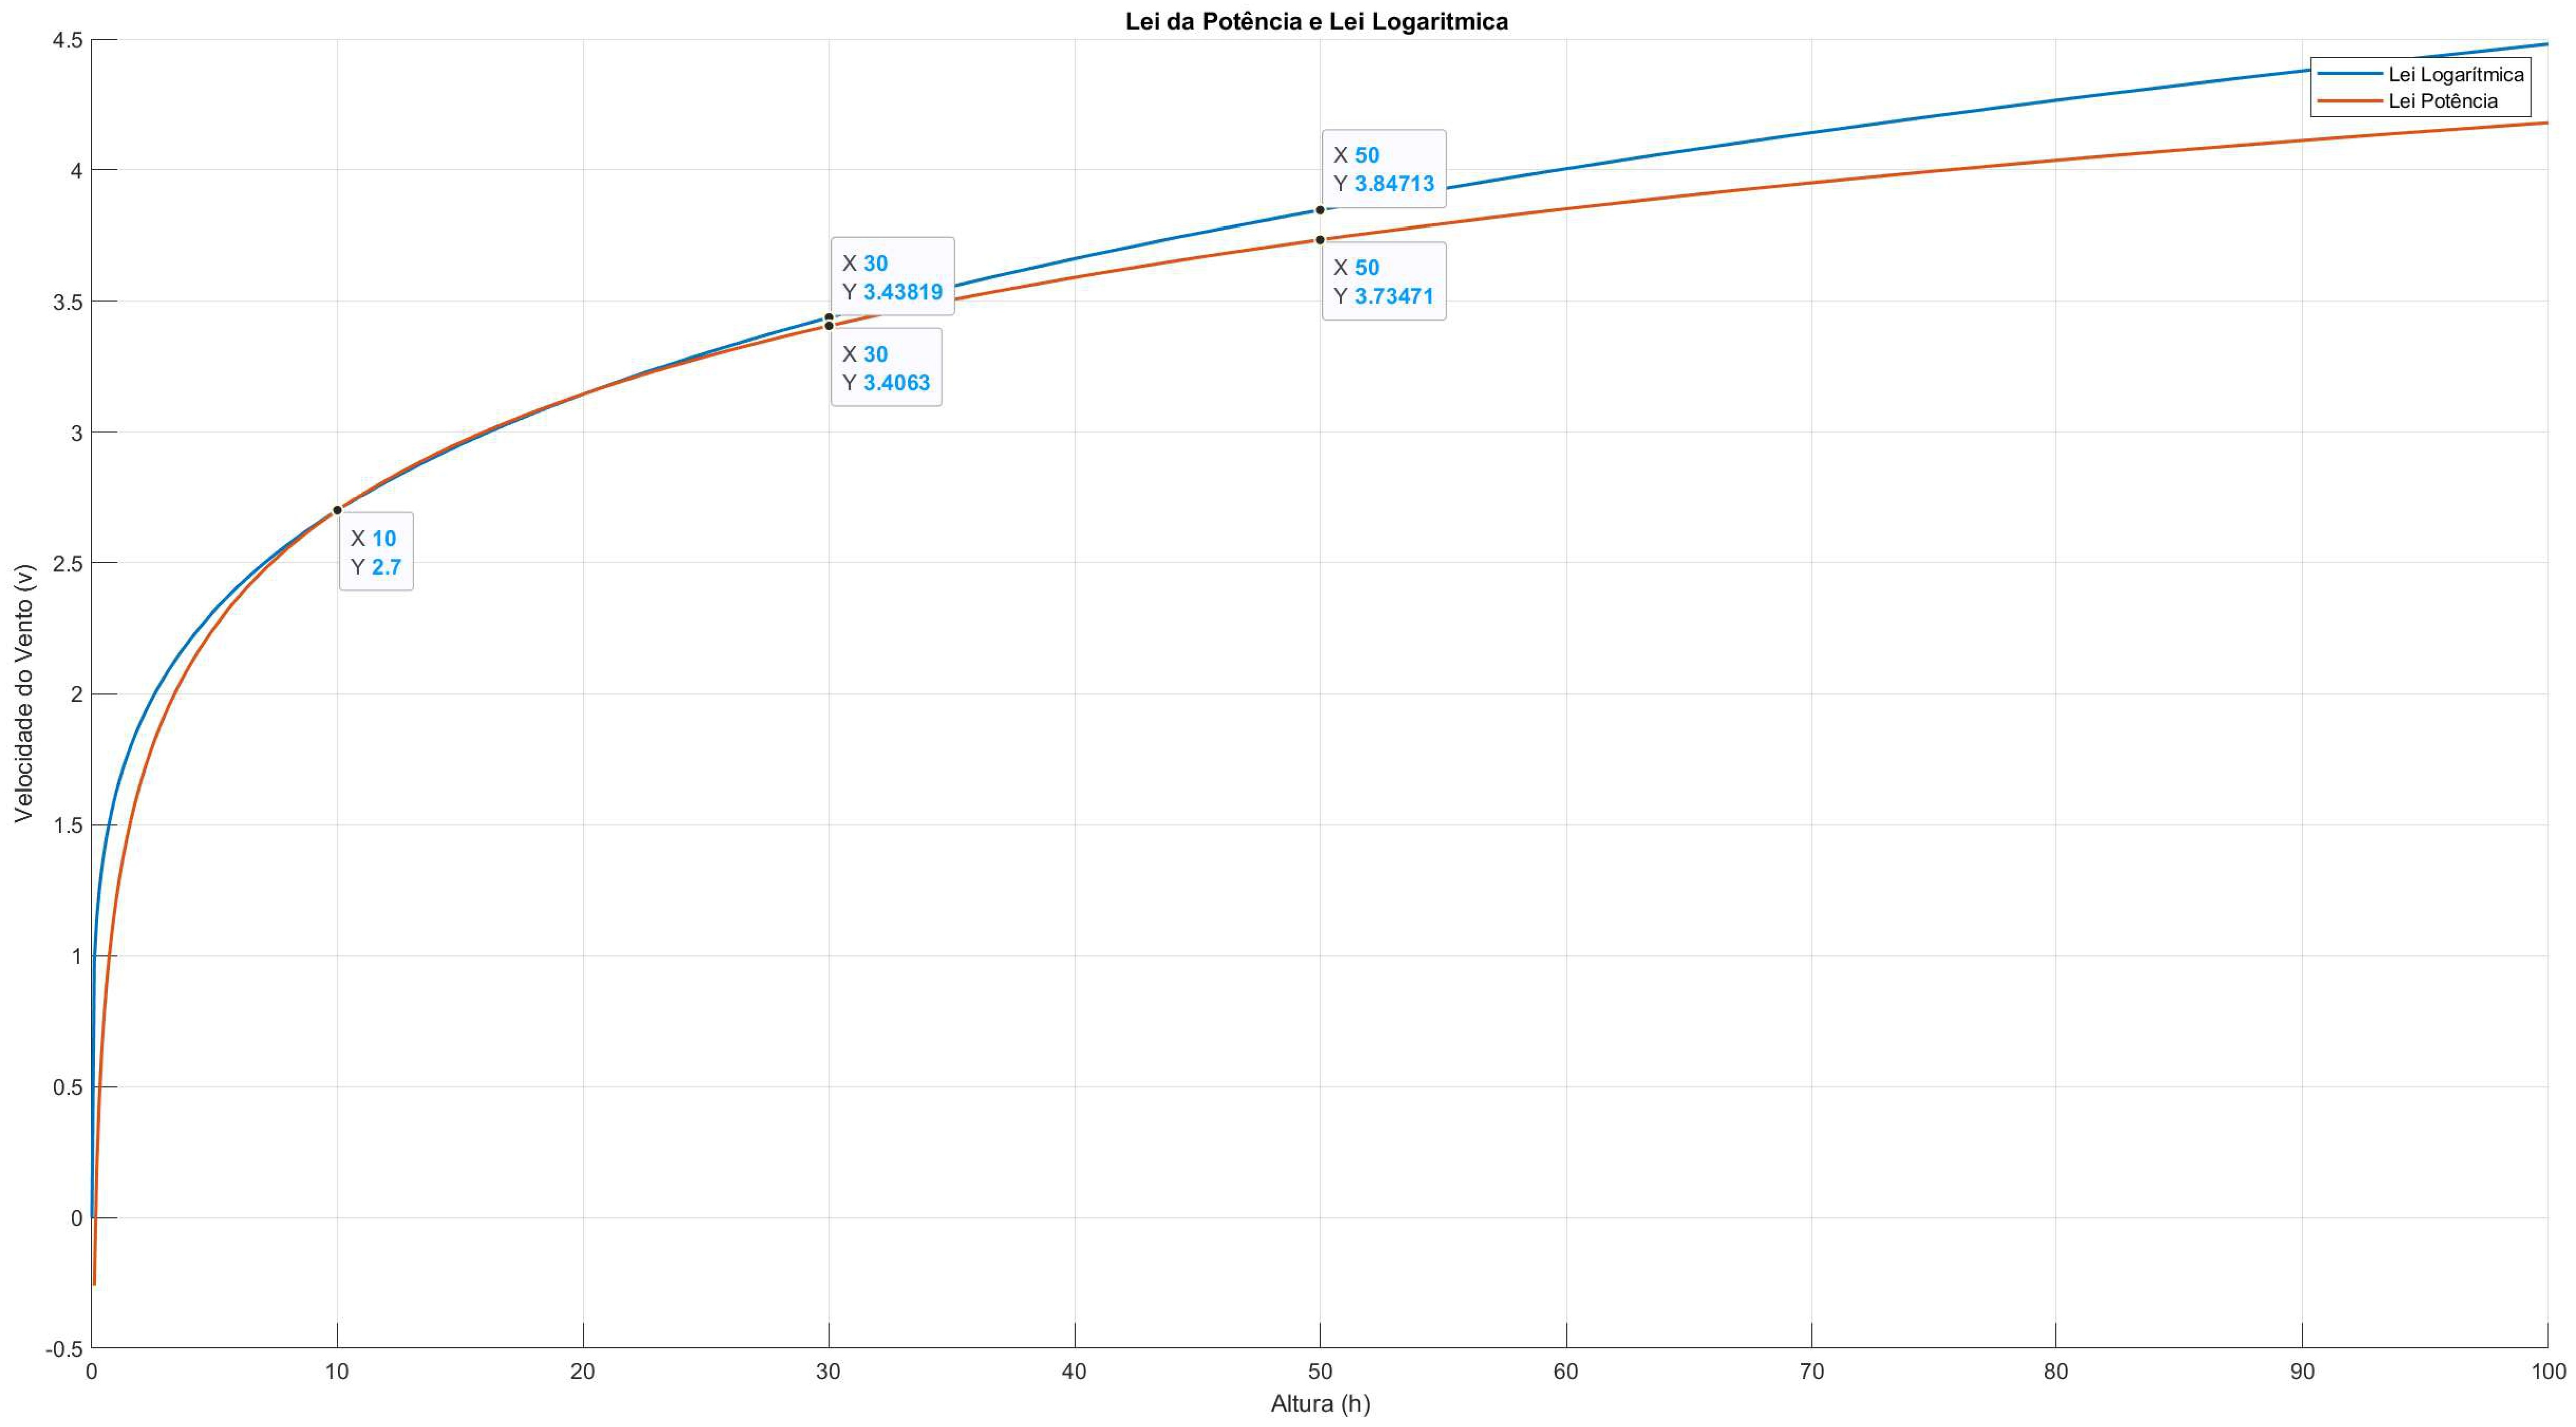
\includegraphics[width=1\textwidth]{Figuras/Teorico/Lei da Potencia e Lei Logaritmica.jpg}
            
        \end{figure}
        
        
        \section{Potência gerada pelos ventos}
        \par O movimento do ar gera energia, conhecida como energia eólica, que é uma forma de energia cinética. Devido à natureza estocástica do vento, sua direção e velocidade variam constantemente. A potência, em termos físicos, é a medida da quantidade de trabalho realizado por unidade de tempo. Para estimar a potência do vento, o processo pode ser dividido em duas etapas: primeiramente, avaliando a energia contida no vento e, em seguida, determinando a fração dessa energia que será convertida em energia mecânica.

        \subsection{Avaliação da Energia Contida no Vento}
        
        Para estimar a energia cinética, iremos inicialmente considerar o exemplo de um cilindro, conforme ilustrado na Figura \ref{fig:Fluxo de massa de ar com velocidade V através de uma área A}. Toda a quantidade de ar que se desloca a uma dada velocidade ($v$) atravessa perpendicularmente o cilindro. 
        %Suponha que a massa de ar que passa pelo cilindro seja $m$.

        \begin{figure}[H]
            \caption{O fluxo de massa de ar com velocidade $v$ através de uma área $A$ (circular).}
            \label{fig:Fluxo de massa de ar com velocidade V através de uma área A}
            \centering
            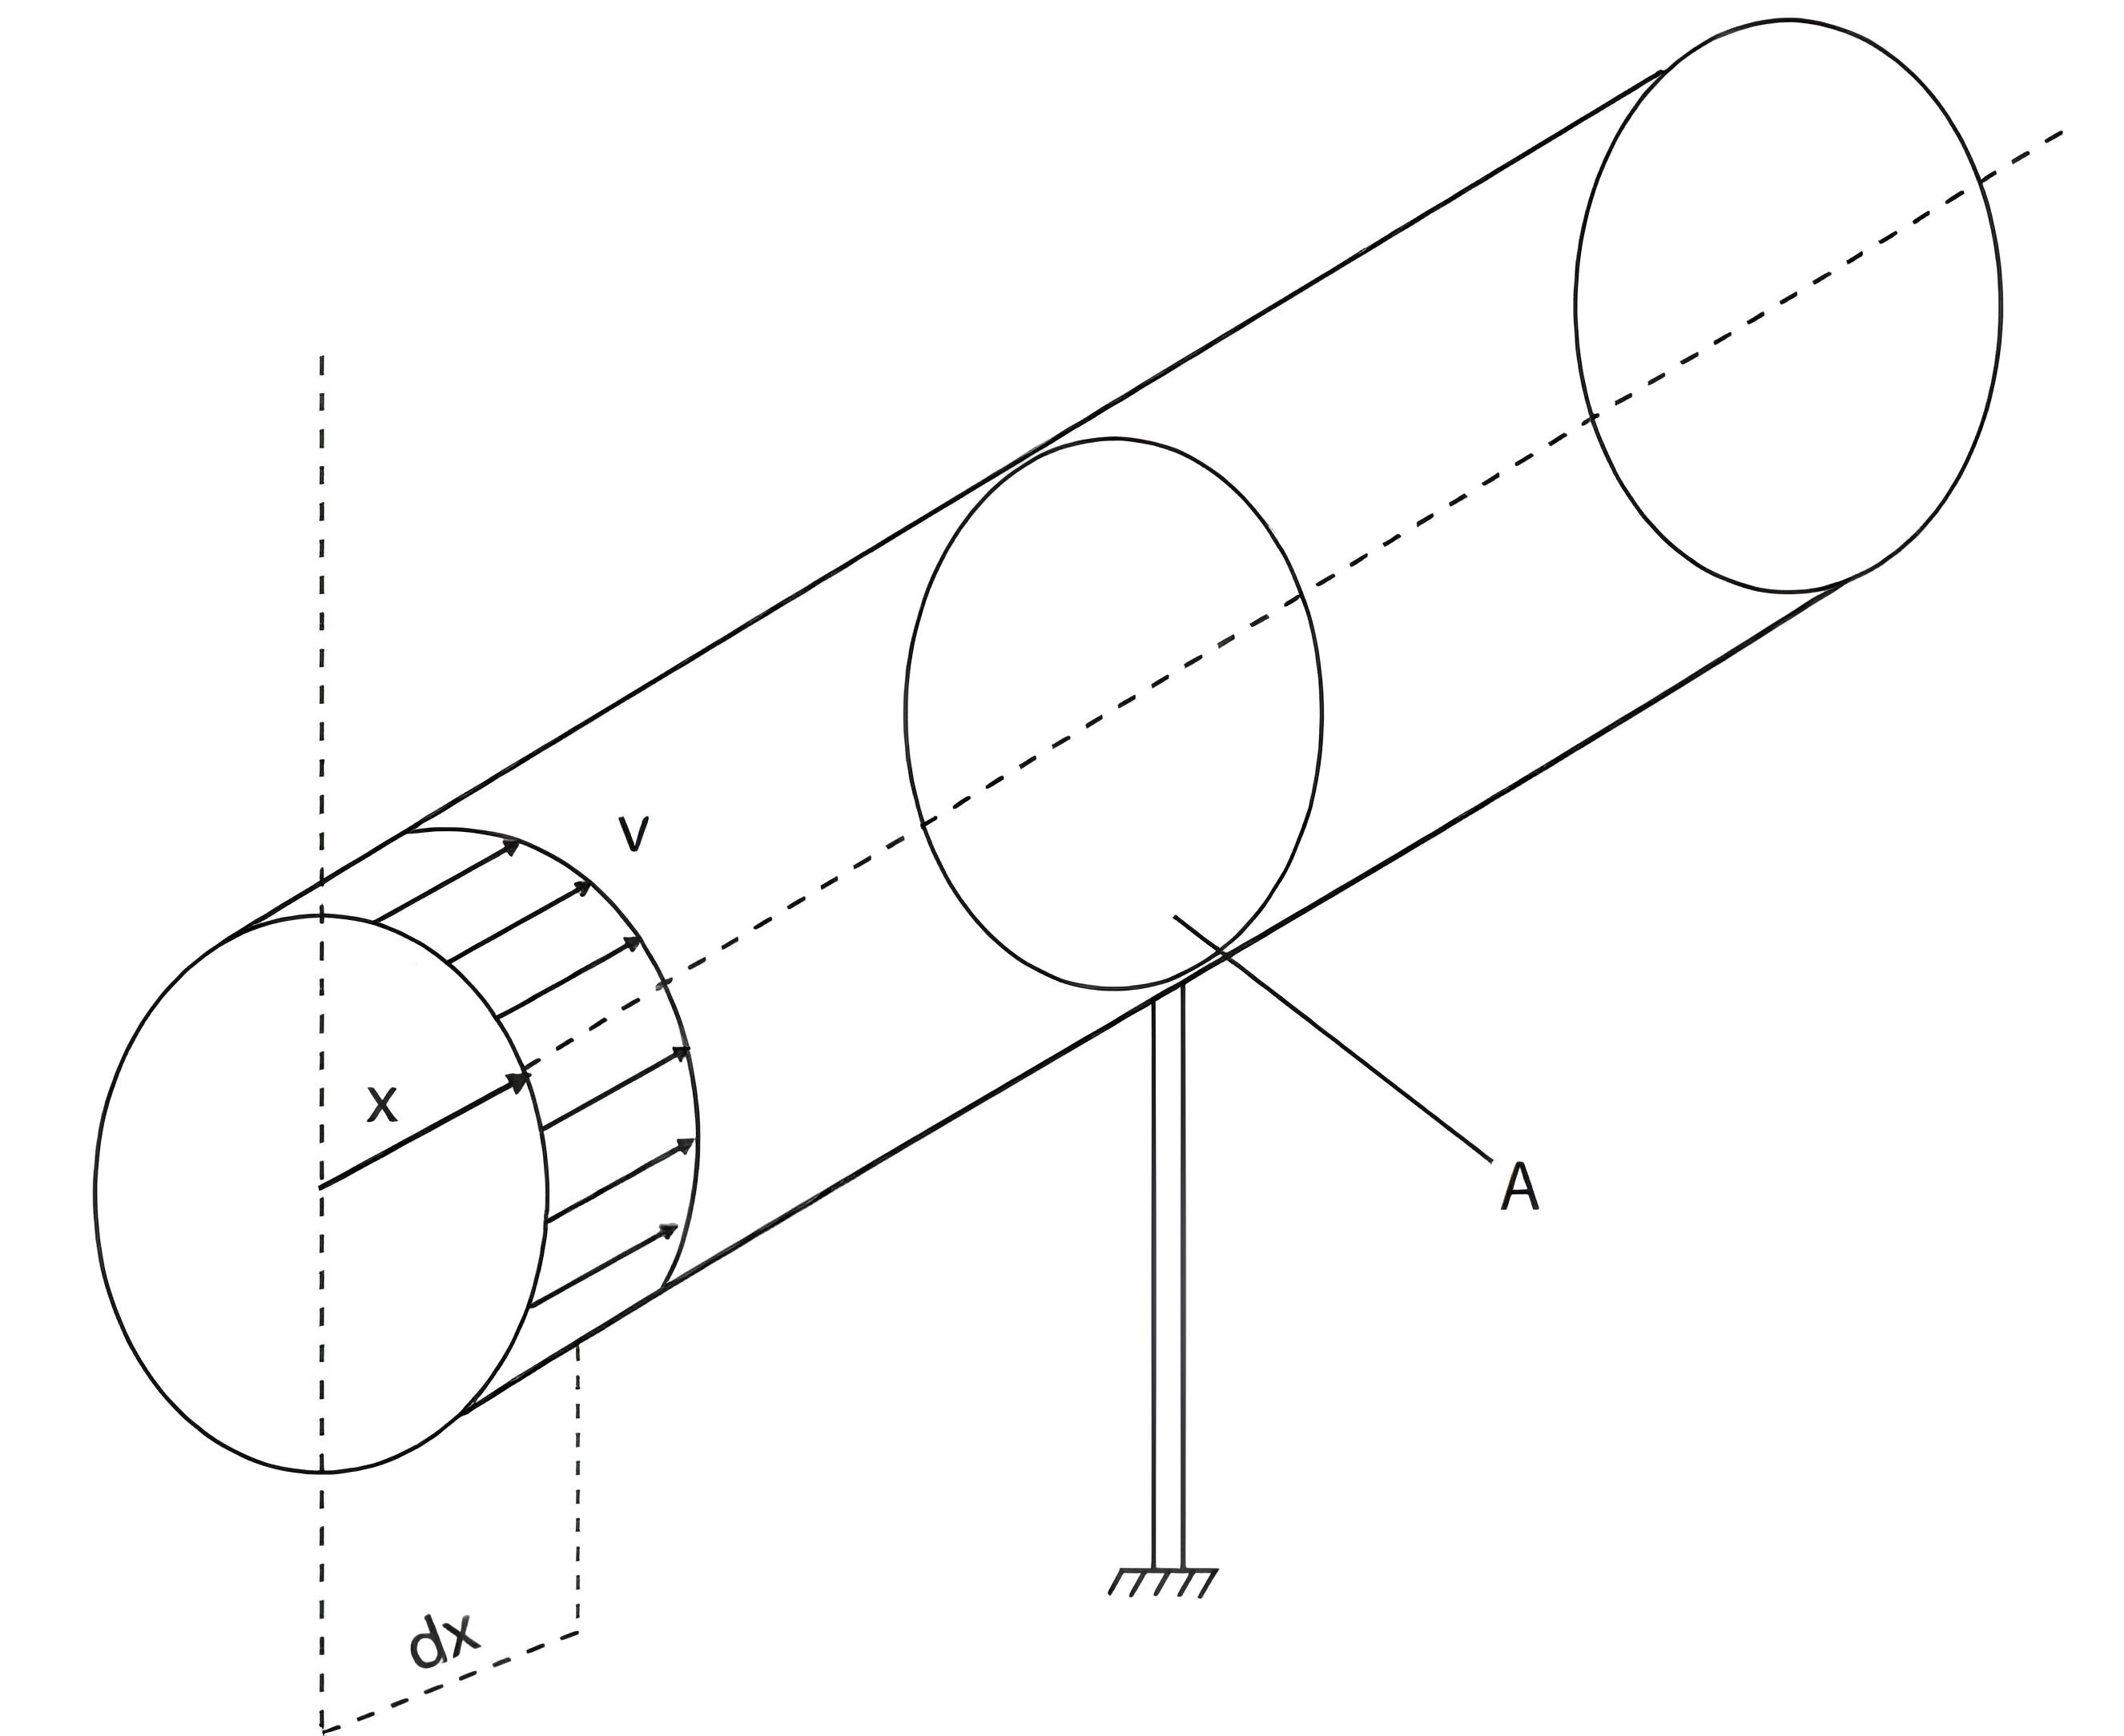
\includegraphics[width=0.5\textwidth]{Figuras/Teorico/Fluxo de massa de ar com velocidade V através de uma área A.jpeg}
            \fonte{\citeonline{carvalho2003}}
        \end{figure}
     
        % \par Consideremos o exemplo de um cilindro ilustrado na Figura \ref{eq:energia cinetica}. Toda a quantidade de ar que se desloca a uma dada velocidade $v$ atravessa perpendicularmente o cilindro. 
        Supondo que a massa de ar que passa pelo cilindro seja $m$, a energia cinética ($E_c$) de uma massa de ar é dada por:
        \begin{equation}
            E_c = \frac{1}{2}mv^2 
            \label{eq:energia cinetica}
        \end{equation}

        \par Essa equação mostra que a energia cinética aumenta com o quadrado da velocidade do vento. Em termos mais simples, ao duplicar a velocidade do vento de um ventilador doméstico, a energia cinética do vento quadruplica. Para encontrar a potência do vento, devemos calcular como essa energia cinética varia ao longo do tempo, o que é feito pela derivada da energia cinética em relação ao tempo. Assim, a potência ($P$) disponível do vento é:

        \begin{equation}
            P = \frac{\partial E_c}{\partial t} = \frac{mv^2}{2} 
            \label{eq:energia cinética ao longo do tempo}
        \end{equation}
        
        \par Para tornar a equação (\ref{eq:energia cinética ao longo do tempo}) mais prática, substitui-se $m$ por $\rho A v$, resultando em
        
        \begin{equation}
            P = \frac{1}{2} \rho A v^3 
            \label{eq:PotênciaVento}
        \end{equation}
        
        \par Essa equação fornece uma boa análise do fluxo de potência eólica. Pode-se também interpretá-la como a quantidade de energia por uma dada área:
        
        \begin{equation}
            \frac{P}{A} = \frac{1}{2} \rho v^3 
            \label{eq:DensidadeDePotência}
        \end{equation}
        sendo as variáveis
        \begin{itemize}
            \item $P$: potência disponível do vento (W)
            \item $m$: fluxo de massa de ar (kg/s)
            \item $\rho$: densidade do ar (kg/m\(^3\))
            \item $A$: área da seção transversal do cilindro atravessada pelo vento (m\(^2\))
            \item $v$: velocidade do vento (m/s)
            \item $E_c$: energia cinética do vento (joules/s)
            \item $\frac{P}{A}$: densidade de potência (W/m\(^2\))
        \end{itemize}
        
        \par A análise da equação (\ref{eq:PotênciaVento}) revela que a potência disponível no vento é diretamente proporcional ao cubo da velocidade do vento. Se a velocidade do vento dobrar, a potência aumentará oito vezes. A densidade de potência $\frac{P}{A}$ representa a potência contida no vento que atinge a parte frontal da turbina. 
        \par A densidade do ar depende da pressão ($P$), da temperatura absoluta ($T$) e da constante do gás ($R$), conforme a equação (\ref{eq:densidadeDoAr}), que para efeitos de analise $\rho = 1.225 \, \text{kg/m}^3$.
        \begin{equation}
            \rho = \frac{P}{R \cdot T}
            \label{eq:densidadeDoAr}
        \end{equation}

        \par Considerando a analise para aplicação de uma turbina eólica de eixo horizontal, como a ilustrada na Figura \ref{fig:turbin_area}, a área varrida pelas pás pode ser determinada a partir da seguinte equação:

        \begin{equation}
            A = \frac{\pi}{4} D^2  \label{eq:ÁreaTurbinaHorizontal}
        \end{equation}    
      em que \textit{D} é o diâmetro do rotor.
        \begin{figure}[h!]
            \centering
            \caption{Área varrida pelas pás de uma turbina de eixo horizontal.}
            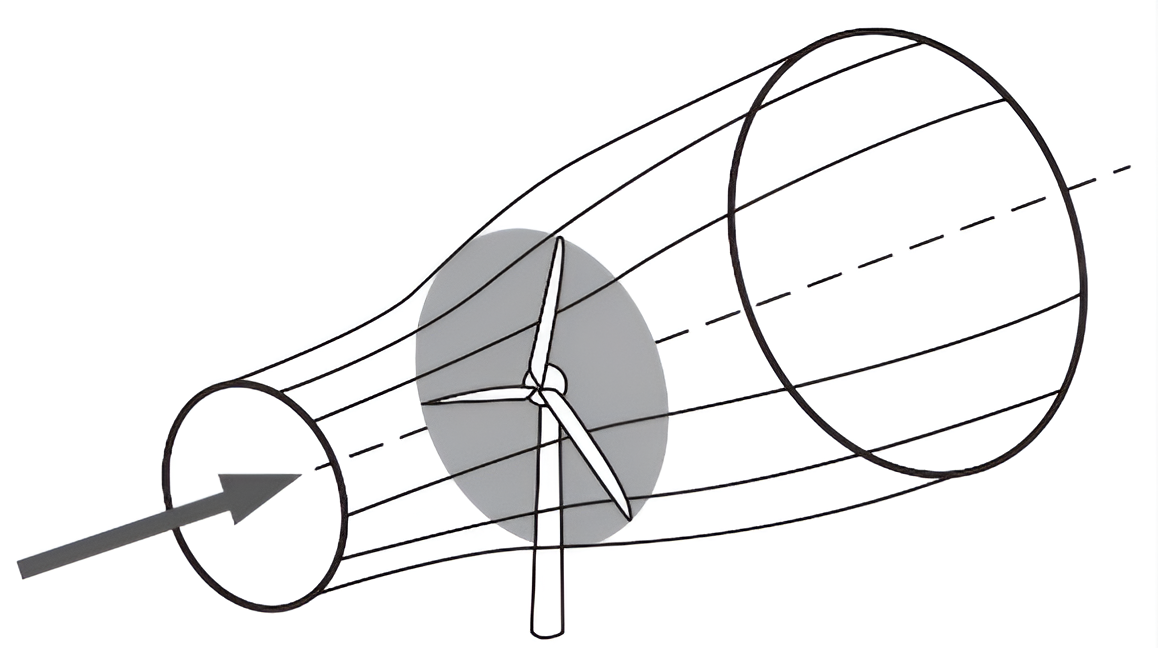
\includegraphics[width=0.7\textwidth]{Figuras/Teorico/areaTurbina.png}
            \label{fig:turbin_area}
            \fonte{\citeonline{fadigas2011} adaptado de \citeonline{burton2001}.}
        \end{figure}

       
        \par A determinação da área para a turbina de eixo vertical modelo Darrieus, mostrada na figura \ref{fig:Darrieus}, é mais complexa, pois envolve integrais elípticas. No entanto, ao aproximar o formato das pás a uma parábola, a seguinte expressão simplificada pode ser utilizada \cite{fadigas2011}:

        \begin{equation}
            A = \frac{2}{3} \cdot (\text{largura máxima do rotor até o centro}) \times (\text{altura do rotor})
        \end{equation}

         \begin{figure}[h!]
            \centering
            \caption{Modelo de Darrieus.}
            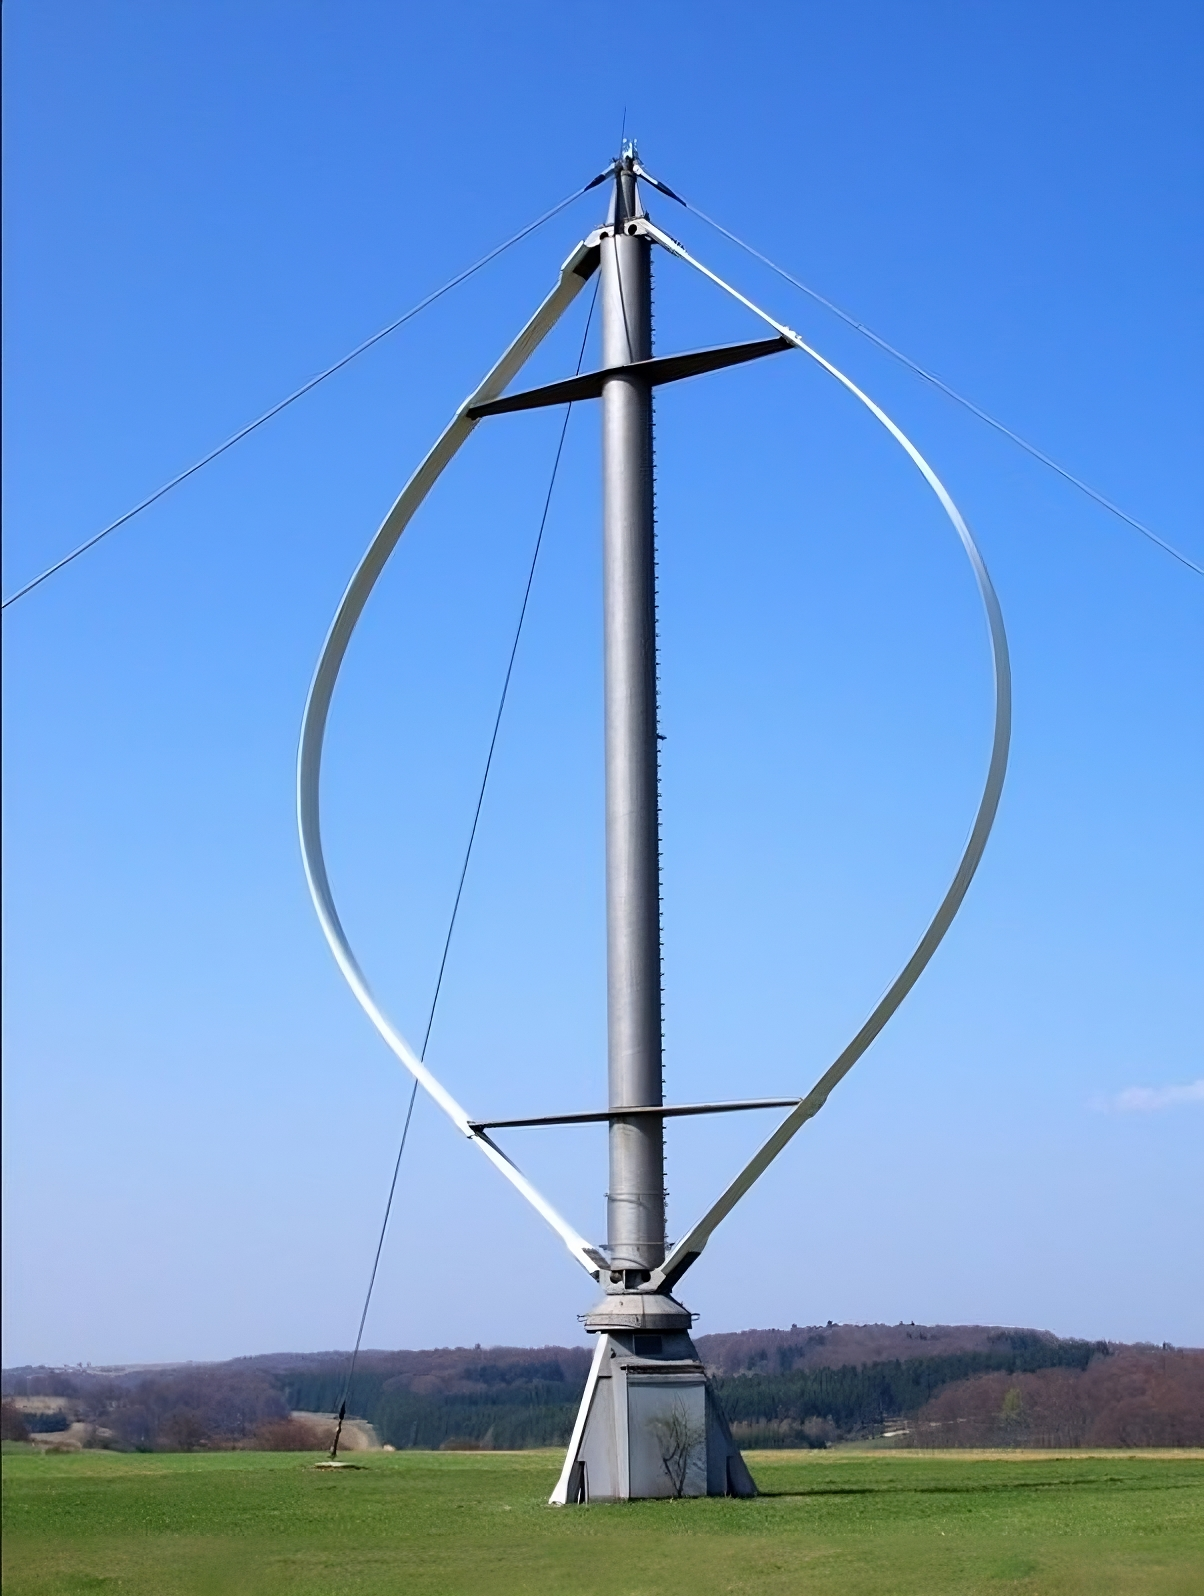
\includegraphics[width=0.5\textwidth]{Figuras/Teorico/modelo Darrieus.jpeg}
            \label{fig:Darrieus}
            \fonte{\citeonline{quora2024}.}
        \end{figure}

        \par Os aspectos mais importantes, destaca \citeonline{fadigas2011}, são que a potência do vento depende da área de captação e é proporcional ao cubo de sua velocidade. Pequenas variações na velocidade do vento podem resultar em grandes mudanças na potência.

        \par A figura \ref{fig:CuboVelocidadeVento} demonstra como a densidade de potência do vento varia com a velocidade. Por exemplo, na figura \ref{fig:CuboVelocidadeVento} é possível ver em destaque para uma velocidade de 8 m/s com a densidade de potência (ao nível do mar) de 314 W/m². Quando a velocidade dobra para 16 m/s, a densidade de potência aumenta para 2.509 W/m², ou seja, oito vezes maior. Isso enfatiza a importância de obter dados altamente precisos.

        \begin{figure}[h!]
            \centering
            \caption{Curva de potência do vento em função de sua velocidade.}
            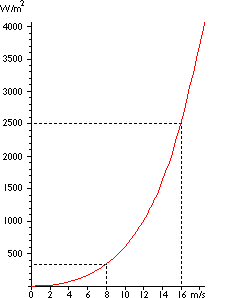
\includegraphics[width=0.4\textwidth, height=0.4\textwidth]{Figuras/Teorico/Cubo de Velocidade do Vento.png}
            \label{fig:CuboVelocidadeVento}
            \fonte{\citeonline{danishwind2024}.}
        \end{figure}

    \subsection{Determinação da Energia Convertida em Potência Mecânica}
    \par A equação (\ref{eq:PotênciaVento}) refere-se a potência contida nos ventos ou potência eólica determinada para um cilindro, em função da massa específica do ar, área de captação e velocidade do vento. Entretanto, nesta estimativa a velocidade não sofre pertubação, ou seja, é uma estimativa de potência antes de atingir as pás do rotor. Em cenário real, esse vento ao encontrar as pás do aerogerador terá o seu perfil modificado, como ressaltado na figura \ref{fig:Passagem de ar por uma turbina eólica de eixo horizontal.}.

        \begin{figure}[h!]
            \centering
            \caption{Passagem de ar por uma turbina eólica de eixo horizontal.}
            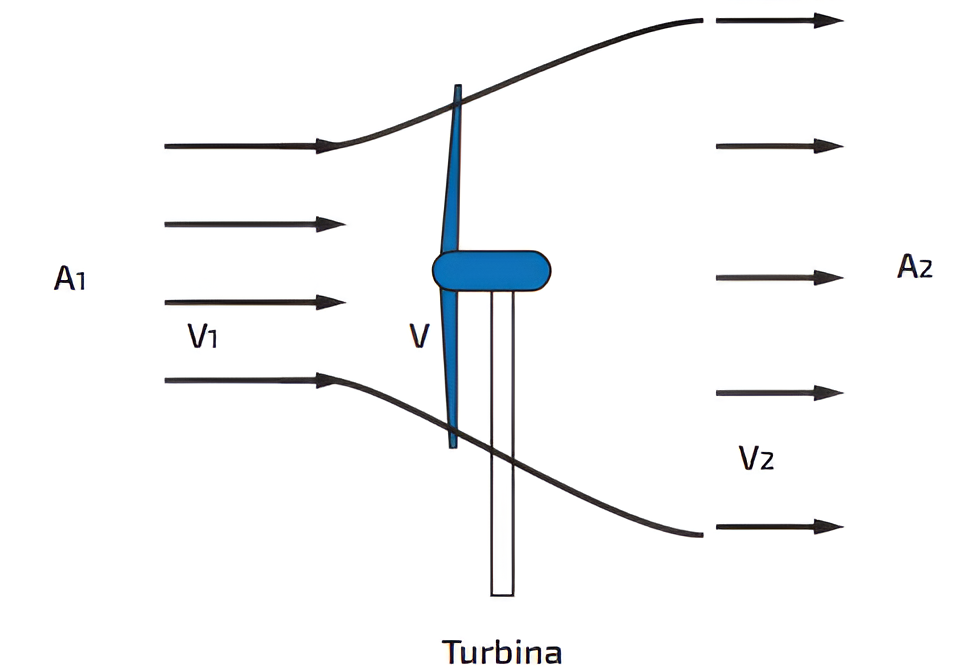
\includegraphics[width=0.4\textwidth, height=0.4\textwidth]{Figuras/Teorico/Fluxo de ar através de uma turbina eólica de eixo horizontal.png}
            \label{fig:Passagem de ar por uma turbina eólica de eixo horizontal.}
            \fonte{\citeonline{rocha2023}.}
        \end{figure}

    \par O vento, ao passar pelo aerogerador, tem uma parte de sua potência convertida em potência mecânica. Como resultado dessa conversão, a velocidade inicial do vento diminui durante a passagem pelo aerogerador, e a área de fluxo de ar aumenta. Utilizando a equação da continuidade, sabemos que o fluxo de massa $\dot{m}$ permanece constante, conforme destacado na equação (\ref{eq:lei de continuidade de fluxo}). Além disso, a potência mecânica ($P_{mec}$) gerada é igual à diferença entre a potência de entrada ($P_{in}$) e a potência de saída ($P_{out}$), conforme expresso na equação (\ref{eq:PotMec_pela_diferenca_Pin_Pout}).
    

    \begin{equation}
        \rho_1 A_1 v_1 = \rho_2 A_2 v_2 = \dot{m} \quad \text{(kg/s)}
        \label{eq:lei de continuidade de fluxo}
    \end{equation}
    
    \begin{equation}
        P_{mec}=P_{in}-P_{out}
        \label{eq:PotMec_pela_diferenca_Pin_Pout}
    \end{equation}
    \par As potências de entrada e saída podem ser expressas a partir de (\ref{eq:PotênciaVento})
    \begin{equation}
        P_{in}=\frac{1}{2} \rho A_1 v_1^3
        \label{eq:PotênciaEntrada}
    \end{equation}
    \begin{equation}
        P_{out}=\frac{1}{2} \rho A_2 v_2^3
        \label{eq:PotênciaSaida}
    \end{equation}
    assim, substituindo em  (\ref{eq:PotMec_pela_diferenca_Pin_Pout}), tem-se
    \begin{equation}
        P_{mec}=\frac{1}{2} \rho A_1 v_1^3 - \frac{1}{2} \rho A_2 v_2^3 =\frac{1}{2} \rho (A_1 v_1^3 - A_2 v_2^3)
        \label{eq:PotMec_Associando_Termos}
    \end{equation}
    em que, a potência mecânica $P_{mec}$ extraída é equivalente à diferença entre o fluxo de ar antes e após a passagem pela turbina. Aplicando a equação da continuidade (\ref{eq:lei de continuidade de fluxo}) em  (\ref{eq:PotMec_Associando_Termos}), obtém-se:
        \begin{equation}
        P_{mec}=\frac{1}{2} \rho A_1 v_1(v_1^2 - v_2^2) = \frac{1}{2} m (v_1^2 - v_2^2)
        \label{eq:PotMec_pela_Eq.Cont.Fluxo}
    \end{equation}
    
\section{Curva Coeficiente de Performance (\(C_{p}\))}
    \par A curva $C_p$, ou curva do coeficiente de potência, é uma representação fundamental na análise de desempenho de turbinas eólicas, ilustrando a eficiência com que uma turbina converte a energia cinética do vento em energia mecânica no eixo da turbina. O coeficiente de potência $C_p$ é adimensional e varia em função da razão de velocidade das pontas das pás $\lambda$ (\textit{tip speed ratio}, TSR), que é uma medida da velocidade linear das pontas das pás relativa à velocidade do vento.

    \par Segundo \citeonline{betz1926}, uma turbina eólica ideal reduz a velocidade do vento a 2/3 da velocidade original, limitando a potência capturável a aproximadamente 59\% da potência total disponível. Esse limite é conhecido como o limite de Betz. Assim aplicando o conceito a equação \ref{eq:PotênciaVento} da potência do extraída do vento, tem-se:
    \begin{equation}
        P_{mec} = \frac{1}{2} C_p \rho A v^3 
    \end{equation}
    o coeficiente de potência em termos isolados:
    \begin{equation}
        C_p = \frac{P_{mec}}{\frac{1}{2} \rho A v^3}
        \label{eq:CoeficienteDePotência}
    \end{equation}
    \begin{itemize}
        \item \( P_{mec} \) representa a potência mecânica produzida pela turbina,
        \item \( \rho \) é a densidade do ar,
        \item \( A \) corresponde à área alcançada pelas pás da turbina,
        \item \( v \) indica a velocidade do vento ao entrar na turbina.
    \end{itemize}
    \par Em turbinas eólicas reais, o coeficiente de performance varia tipicamente de acordo com o TSR ($\lambda$), dada pela equação, e o ângulo de passo das pás. 
    \begin{equation}
        \lambda = \frac{\omega R}{v}
        \label{eq:lambda}
    \end{equation}
    sendo que
    \begin{itemize}
        \item \( \omega \): representa a velocidade angular do rotor, medida em radianos por segundo [rad/s],
        \item \( R \): indica o raio das pás do rotor, em metros [m],
        \item \( v \): denota a velocidade do vento, em metros por segundo [m/s].
    \end{itemize}
   

    \par O comportamento da curva Cp é influenciado pela aerodinâmica das pás, pelas características do rotor, e pelas condições operacionais da turbina. Em turbinas com controle ativo de passo, o ângulo das pás ($\beta$) é ajustado para maximizar $C_p$ para diferentes velocidades do vento e para proteger a turbina em condições de vento forte.

    \par Modelos matemáticos, como os desenvolvidos por \citeonline{heier2014} e por \citeonline{slootweg2003}, utilizam séries de equações, (\ref{eq:lambda}) - (\ref{eq:Cp(lambda,beta)}), para estimar $C_p$ em função do TSR e do ângulo de passo das pás ($\beta$). Esses modelos são cruciais para o design otimizado e a operação eficiente de turbinas eólicas, permitindo que operadores e designers ajustem as turbinas para operar próximo ao máximo coeficiente de performance sob várias condições de vento.

    \begin{equation}
        C_p(\lambda, \beta) = c_1 \left( \frac{c_2}{\lambda_i} - c_3 \beta - c_4 \beta c_5 - c_6 \right) e^{-\frac{c_7}{\lambda_i}} 
        \label{eq:Cp(lambda,beta)}
    \end{equation}
        
    \begin{equation}
        \lambda_i = \frac{1}{\frac{1}{\lambda + c_8 \beta} -\frac{c_9}{\beta^3 + 1}}
        \label{eq:lambdai}
    \end{equation}

    \par $\beta$ é  o ângulo de passo das pás.
    \par $\lambda$ é o coeficiente de velocidade.

    \par Os coeficientes $c_i$ estão delineados na Tabela \ref{tab:parametros}, conforme descrito por \citeonline{heier2014}, \citeonline{slootweg2003} e \citeonline{raiambal2002modeling}. A metodologia para estimar a eficiência aerodinâmica sugerida por Heier e Raiambal é aplicável universalmente, abrangendo tanto turbinas de velocidade fixa quanto variável. Por outro lado, \citeonline{slootweg2003} adaptaram os parâmetros nas equações (\ref{eq:Cp(lambda,beta)}) e (\ref{eq:lambdai}) para refletir as particularidades dessas duas categorias de turbinas eólicas, permitindo uma representação mais precisa das curvas de desempenho em simulações computacionais.

    \begin{table}[H]
        \centering
        \caption{Valores propostos para os parâmetros de cálculo do $C_p(\lambda, \beta)$}
        \label{tab:parametros}
        \begin{tabular}{@{}lccccccccc@{}}
            \toprule
                              & $c_1$ & $c_2$ & $c_3$ & $c_4$ & $c_5$ & $c_6$ & $c_7$ & $c_8$ & $c_9$ \\ \midrule
            Heier             & 0.5   & 116   & 0.4   & 0     & -     & 5     & 21    & 0.08  & 0.035 \\
            Raiambal             & 0.5   & 116   & 0.4   & 0     & -     & 5     & 16.5    & 0.089  & 0.035 \\
            Velocidade Constante & 0.44  & 125   & 0     & 0     & 0     & 6.94  & 16.5  & 0     & -0.002\\
            Velocidade Variável  & 0.73  & 151   & 0.58  & 0.002 & 2.14  & 13.2  & 18.4  & -0.02 & -0.003\\ \bottomrule
        \end{tabular}
            \begin{flushleft}
                \footnotesize{Fonte: \citeonline{vian2021}.}
            \end{flushleft}
    \end{table}

    \par Inserindo os valores da Tabela \ref{tab:parametros} em (\ref{eq:Cp(lambda,beta)}) e (\ref{eq:lambdai}), tem-se conforme  \citeonline{heier2014}
    \begin{equation}
        C_p(\lambda, \beta) = 0.5 \left( \frac{116}{\lambda_i} - 0.4 \beta - 5 \right) e^{-\frac{21}{\lambda_i}} 
        \label{eq:Cp(lambda,beta) Heier}
    \end{equation}
   
    \begin{equation}
        \lambda_i = \frac{1}{\frac{1}{\lambda + 0.08 \beta} -\frac{0.035}{\beta^3 + 1}}
        \label{eq:lambdai Heier}
    \end{equation}
    
    De acordo com \citeonline{raiambal2002modeling}, obtêm-se
        \begin{equation}
        C_p(\lambda, \beta) = 0.5 \left( \frac{116}{\lambda_i} - 0.4 \beta - 5 \right) e^{-\frac{16.5}{\lambda_i}} 
        \label{eq:Cp(lambda,beta) Raiambal}
    \end{equation}
   
    \begin{equation}
        \lambda_i = \frac{1}{\frac{1}{\lambda + 0.089} -\frac{0.035}{\beta^3 + 1}}
        \label{eq:lambdai Raiambal}
    \end{equation}
     
    Por fim, para os paramentos estabelecidos por \citeonline{slootweg2003}, tem-se para velocidade variável

    \begin{equation}
        C_p(\lambda, \beta) = 0.73 \left( \frac{151}{\lambda_i} - 0.58 \beta - 0.002 \beta^{2.14} - 13.2 \right) e^{-\frac{18.4}{\lambda_i}} 
        \label{eq:Cp(lambda,beta) Slootweg}
    \end{equation}
        
    \begin{equation}
        \lambda_i = \frac{1}{\frac{1}{\lambda -0.02 \beta} -\frac{-0.003}{\beta^3 + 1}}
        \label{eq:lambdai Slootweg}
    \end{equation}

    \par Nas figuras \ref{fig:graph1}, \ref{fig:graph2} e \ref{fig:graph3}, são apresentadas as curvas de potência para três metodologias de eficiência diferentes, simuladas via script no MATLAB para a turbina do projeto. A análise dos gráficos destacou a eficiência típica de 45\% para aerogeradores horizontais de três pás, valor comumente observado em turbinas desse tipo \cite{smartservo2024}.

    \begin{figure}[H]
        \centering
        \caption{Coeficiente de Potência ($C_p$) versus Relação de Velocidade na Ponta ($\lambda$) para ângulo de passo $\beta$, para equações (\ref{eq:Cp(lambda,beta) Raiambal}) e (\ref{eq:lambdai Raiambal}).}
        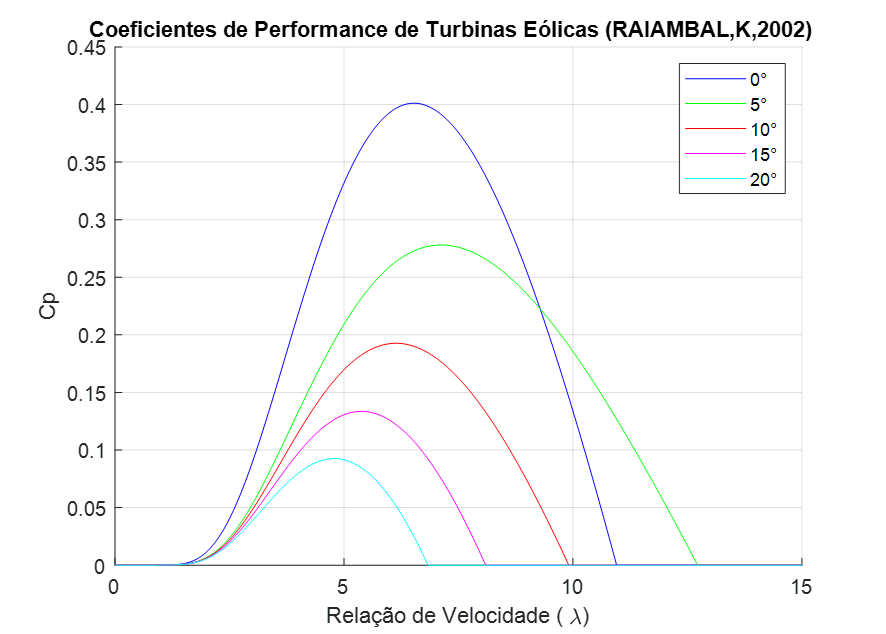
\includegraphics[width=0.6\textwidth]{Figuras/Teorico/graph1.png} % Substitua pelo caminho correto
        \label{fig:graph1}
    \end{figure}
    
    \begin{figure}[H]
        \centering
        \caption{Coeficiente de Potência ($C_p$) versus Relação de Velocidade na Ponta ($\lambda$) para ângulo de passo $\beta$, para equações (\ref{eq:Cp(lambda,beta) Slootweg}) e (\ref{eq:lambdai Slootweg}).}
        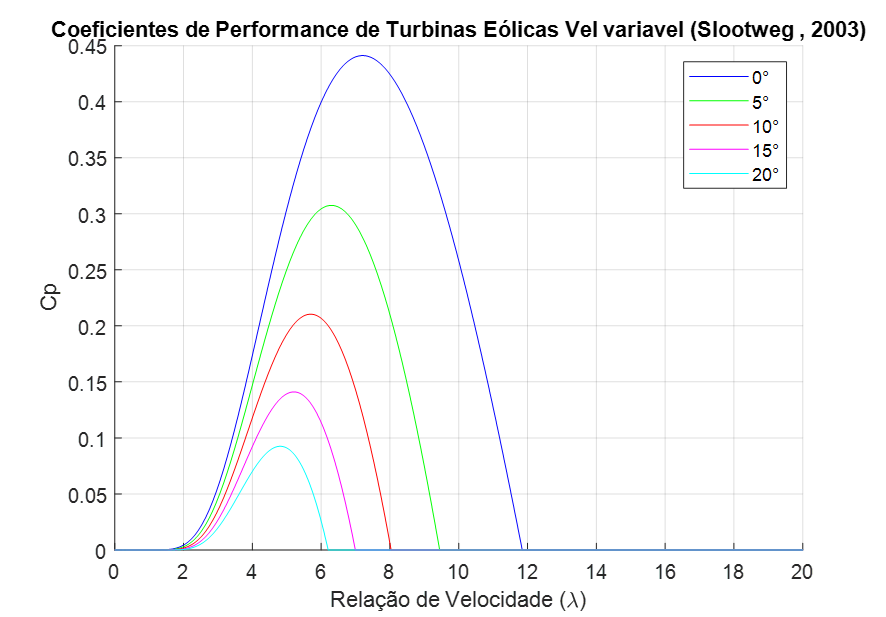
\includegraphics[width=0.6\textwidth]{Figuras/Teorico/graph2.png} % Substitua pelo caminho correto
        \label{fig:graph2}
    \end{figure}
    
    \begin{figure}[H]
        \centering
        \caption{Coeficiente de Potência ($C_p$) versus Relação de Velocidade na Ponta ($\lambda$) para ângulo de passo $\beta$, para equações (\ref{eq:Cp(lambda,beta) Heier}) e (\ref{eq:lambdai Heier}).}
        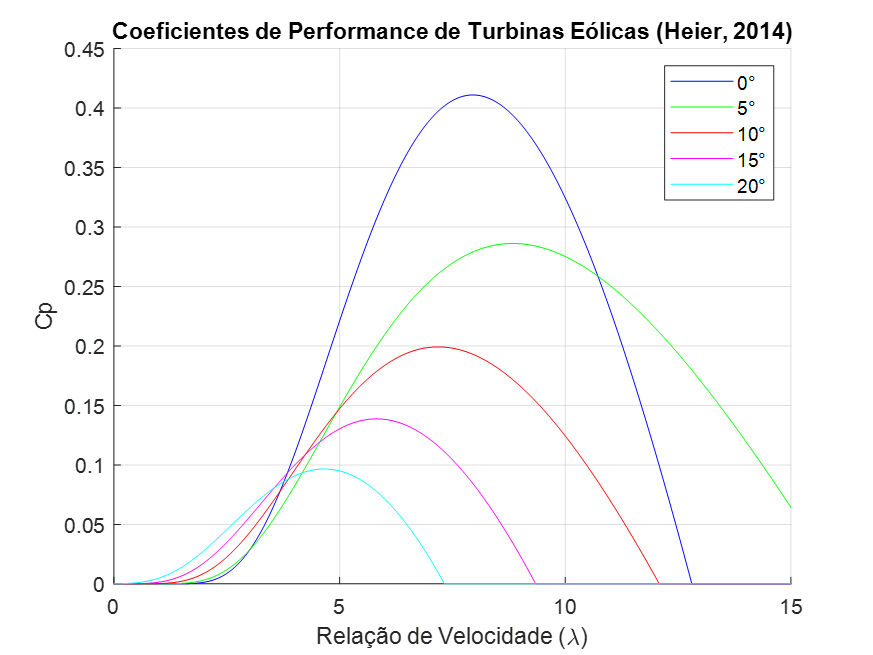
\includegraphics[width=0.6\textwidth]{Figuras/Teorico/graph3.png} % Substitua pelo caminho correto

        \label{fig:graph3}        
    \end{figure}
    
\section{Série Temporal do Vento}


\par Neste capitulo será apresentado a modelagem da série temporal de vento. Tal implementação torna-se necessária pois a série temporal de vento representa a variação da velocidade e seu comportamento ao longo do tempo. Toda a modelagem e simulação foi feita com o uso do software MATLAB/SIMULINK. O desenvolvimento da série temporal será dividido em duas partes: Vento e Fluxo e a Modelagem de Séries Temporais com o Filtro de Von Karman.

\par As séries temporais de vento são registros contínuos da velocidade e direção do vento que desempenham um papel crucial no processo de conversão eólica. Essas séries permitem a análise de padrões históricos e a previsão de flutuações futuras essenciais para a operação eficiente de aerogeradores. A abordagem 'Vento e Fluxo' divide o vento em categorias, facilitando a compreensão dos comportamentos ruidosos presentes nele. Na próxima seção será abordado o passo a passo para a representação da série temporal.

\subsection{Vento e Fluxo}

\par Dividir o fluxo de vento em categorias, como vento médio, turbulência e ondas, ajuda a entender e prever o comportamento do vento sob diversas condições atmosféricas. Cada uma dessas categorias pode ocorrer isoladamente ou simultaneamente, influenciando de maneira distinta a camada limite atmosférica, onde ocorre o transporte de calor, umidade e poluentes. A representação das três categorias pode ser vista na figura \ref{fig:fluxo_ar}. 

\begin{figure}[h]
    \centering
    \caption{Fluxo de ar decomposto em três categorias. \(U\) é o componente velocidade do vento ao longo do tempo \(t\).}
    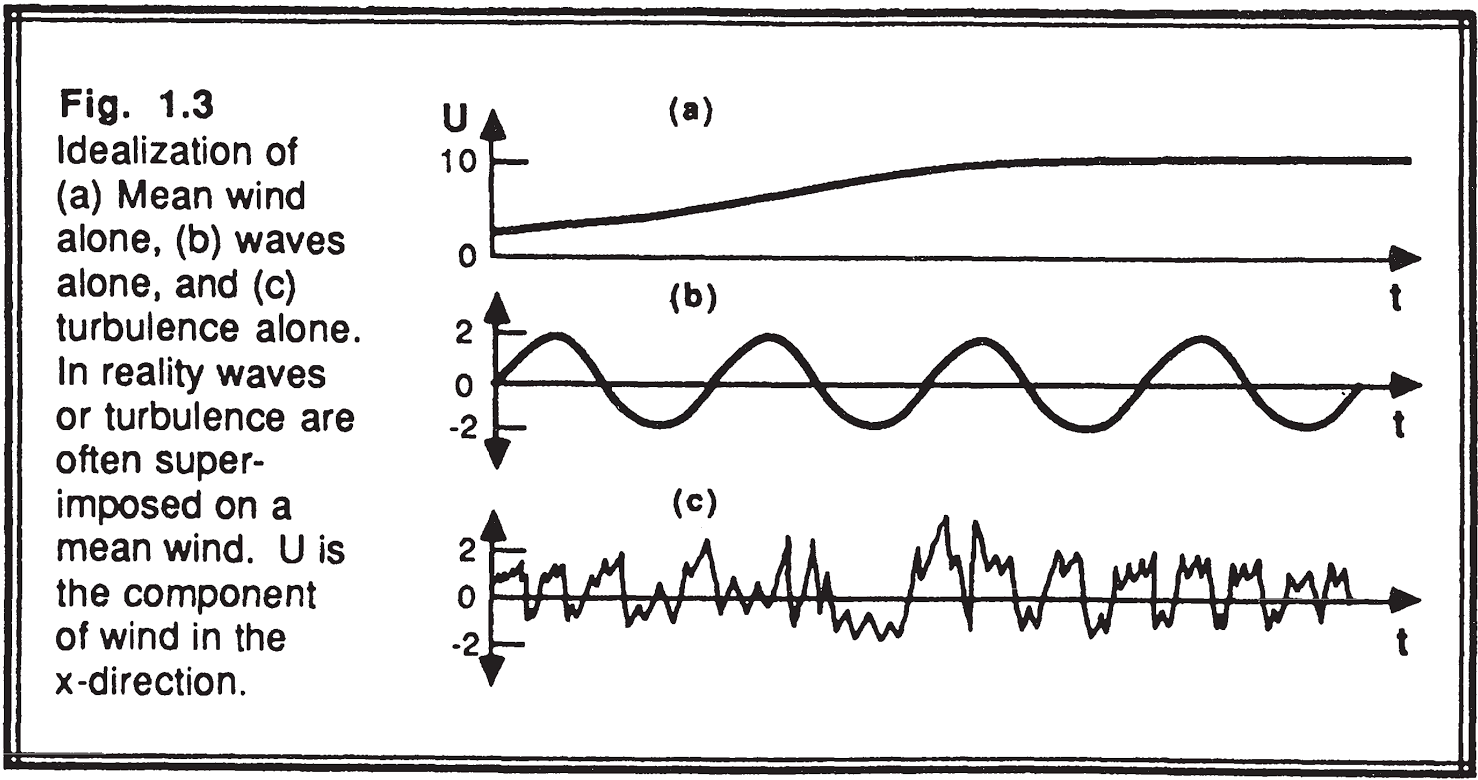
\includegraphics[width=\textwidth]{Figuras/Teorico/vento_sub3_fonte.png}
    \label{fig:fluxo_ar}
    \fonte{\cite{stull1988}}
\end{figure}


\begin{itemize}
    \item \textbf{Vento Médio}
    \begin{itemize}
        \item \textbf{Transporte Horizontal Rápido (Advecção):} O vento médio é responsável por um transporte horizontal muito rápido conhecido como advecção, que é crucial para a movimentação de massas de ar e suas propriedades dentro da camada limite.
        \item \textbf{Velocidade do Vento:} Na camada limite, ventos horizontais variam geralmente entre 2 e 10 m/s. Esses ventos são essenciais para a dispersão de poluentes e o transporte de calor e umidade.
        \item \textbf{Influência da Fricção:} A fricção com a superfície da Terra reduz a velocidade do vento médio perto do solo. Esta redução é mais pronunciada nas proximidades do solo devido ao aumento do arrasto friccional.
    \end{itemize}
    
    \item \textbf{Ondas}
    \begin{itemize}
        \item \textbf{Presença na Camada Limite Noturna:} Ondas atmosféricas são frequentemente observadas durante a noite na camada limite. Elas se formam devido a variações de temperatura e vento e podem se propagar a partir de fontes distantes como tempestades ou explosões.
        \item \textbf{Transporte de Calor e Poluentes:} Embora as ondas transportem pouco calor, umidade e outros escaladores (como poluentes), são muito eficazes no transporte de momento e energia.
        \item \textbf{Geração de Ondas:} Essas ondas podem ser geradas localmente por cisalhamentos do vento médio ou pelo fluxo de ar sobre obstáculos como montanhas ou edifícios. Elas podem se propagar a partir de fontes distantes e influenciar a dinâmica da camada limite.
    \end{itemize}
    
    \item \textbf{Turbulência}
    \begin{itemize}
        \item \textbf{Caracterização:} A turbulência é visualizada como redemoinhos irregulares, chamados vórtices, e é um fenômeno superposto ao vento médio. Ela consiste em muitos vórtices de tamanhos diferentes que se sobrepõem.
        \item \textbf{Geração de Turbulência:} Grande parte da turbulência na camada limite é gerada por forças no solo como o aquecimento solar do solo, que cria termas de ar quente que sobem, e o arrasto friccional do ar ao passar sobre o solo. Obstáculos como árvores e edifícios também podem defletir o fluxo de ar, criando áreas de turbulência adjacentes e a jusante dos obstáculos.
        \item \textbf{Espectro de Turbulência:} A intensidade relativa dos diferentes vórtices define o espectro de turbulência, que descreve a distribuição de energia entre os vórtices de diferentes tamanhos.
    \end{itemize}
\end{itemize}

\par Individualmente, cada categoria representa um efeito, ação ou força que atua sobre o fluxo de ar. Esta subdivisão do vento permite gerar uma representação matemática do vento ruidoso. Assim, de acordo com o comportamento, é possível estipular as seguintes equações:

\begin{equation}
 v_{\text{vento turbulento}} = \sqrt{-2 \ln x_1}
 \label{eq:ventoTurbulento}
\end{equation}

\begin{equation}
v_{\text{vento ondulante}} = \sin(2\pi x_2)
\label{eq:ventoOndulante}
\end{equation}

\par Representado no MATLAB/SIMULINK nos gráficos da Figura \ref{fig:Vento_sub3}.

\begin{figure}[h]
    \caption{Representação do vento em velocidade média, ondulação e turbulência.}
    \centering
    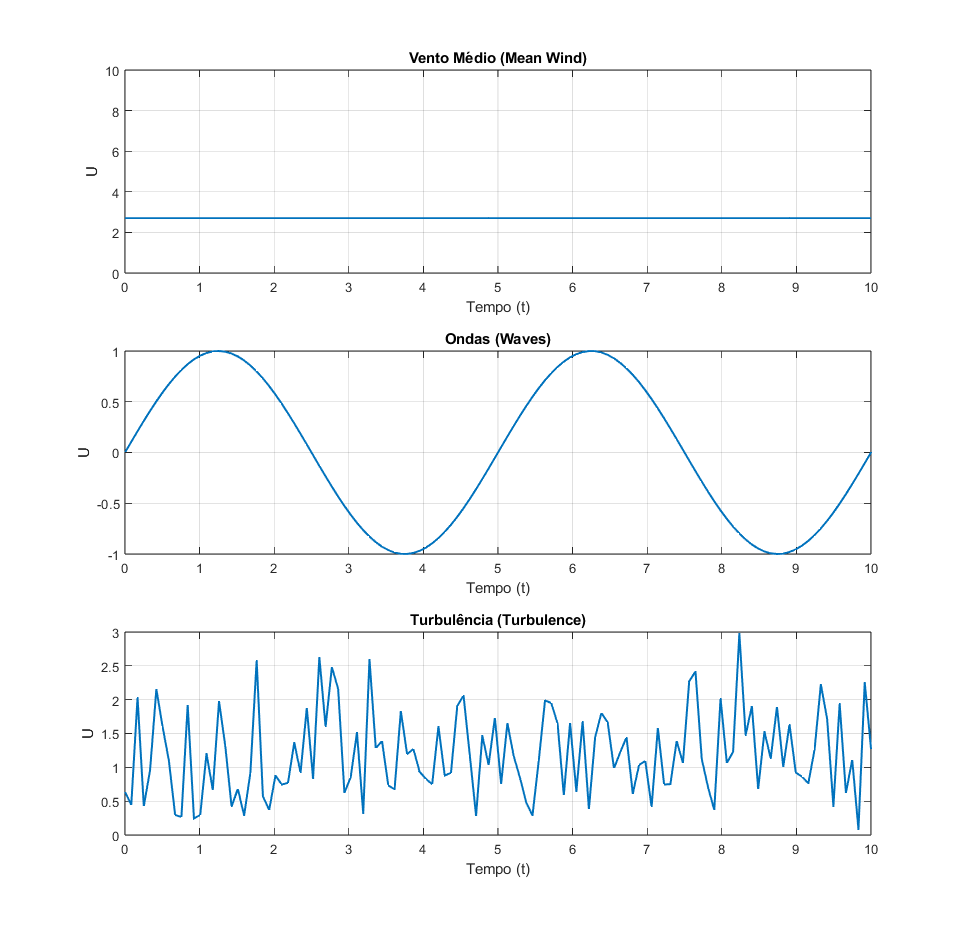
\includegraphics[width=\textwidth]{Figuras/Teorico/vento_sub3.png}
    \label{fig:Vento_sub3}
\end{figure}

\subsection{Modelagem de Séries Temporais com o Filtro de Von Karman}

\par Para modelar adequadamente as séries temporais do vento, é comum utilizar técnicas estatísticas e matemáticas, como o filtro de Von Karman, que ajuda a simular a turbulência do vento. Este filtro é especialmente útil para representar as características caóticas e não lineares do vento, que são críticas para a precisão das simulações. Baseando-se em \citeonline{koch2010} para o desenvolvimento do modelo.

\par Para efeito de análise, podemos considerar que a série temporal do vento é composta por dois termos: um constante e outro variável, sendo respectivamente a velocidade média do vento (\(v\)) e a série temporal de turbulência do vento (\(v_{t}\)):
\begin{equation}
 v(t) = v + v_{t}   
 \label{eq:série temporal do vento}
\end{equation}


\par A parcela que representa a série temporal de turbulência do vento \(v_{t}\) pode ser calculada utilizando o filtro de Von Karman, que é expresso pela função de transferência:

\begin{equation}
G_{Karman}(s) = \frac{K_f}{(1 + sT_f)^{5/6}}
\end{equation}

Onde:
\begin{itemize}
    \item \(K_f\) é o ganho do filtro;
    \item \(T_f\) é a constante de tempo.
\end{itemize}

\par Quando ativado por uma fonte de ruído gaussiano normalizado, a aproximação do filtro de Von Karman por meio de uma função de transferência racional se torna prática. A equação (\ref{eq:Aprox_Filtro_VonKarman}) e a Figura \ref{fig:Aprox_Filtro_VonKarman} representam esta aproximação.

\begin{equation}
G'_{karman}(s) = K_f \frac{(m_1 T_f s + 1)}{(T_f s + 1)(m_2 T_f s + 1)}
\label{eq:Aprox_Filtro_VonKarman}
\end{equation}
sendo os valores das constantes de Von Karman, dados por
\begin{itemize}
    \item \(m_1 = 0.4\);
    \item \(m_2 = 0.25\).
\end{itemize}

\begin{figure}[h]
    \centering
    \caption{Aproximação do Filtro de Von Karman no \textit{software} MATLAB/SIMULINK}
    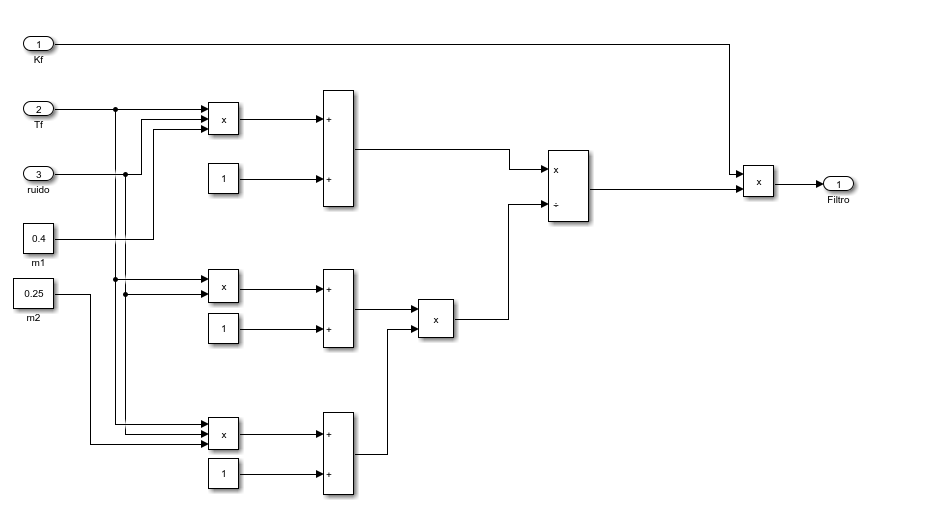
\includegraphics[width=\textwidth]{Figuras/Teorico/Aprox_Filtro_VonKarman.png}
    \label{fig:Aprox_Filtro_VonKarman}
    
\end{figure}

\par Segundo \citeonline{stannard2007performance}, a constante de tempo \(T_f\) está vinculada às especificidades do ambiente onde a turbina está instalada e varia inversamente com a velocidade média do vento conforme a equação:

\begin{equation}
T_f = \frac{L_{turb}}{v}
\label{eq:Constante_Tempo_Tf}
\end{equation}

\par Aqui, \(L_{turb}\) refere-se ao comprimento de turbulência, um fator influenciado pelas características físicas do terreno que não dependem do tipo de turbina utilizada. A determinação precisa de \(L_{turb}\) pode ser complexa devido à necessidade de considerar múltiplos fatores ambientais e topográficos.

\par Para simplificar essa estimativa, \citeonline{martins2010} propôs uma aproximação prática em que \(L_{turb}\) pode ser calculado como 6.5 vezes a altura da torre da turbina \(h\). Assim, pode-se dizer que:

\begin{equation}
L_{turb} = 6.5h
\label{eq:Comprimentodaturbina_aproxMartins}
\end{equation}
representado na Figura \ref{fig:cal_constante_tempoTf}.

\begin{figure}[h]
    \centering
    \caption{Calculo da constante de tempo $T_f$ do Filtro simulado no \textit{software} MATLAB/SIMULINK}
    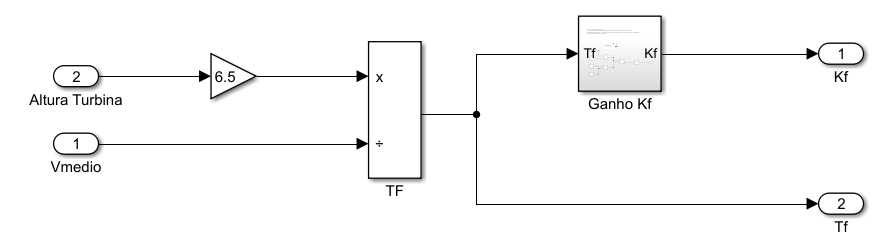
\includegraphics[width=\textwidth]{Figuras/Teorico/constante_de_tempoTf.png}
    \label{fig:cal_constante_tempoTf}
    
\end{figure}


\par O coeficiente \(K_f\), conhecido como ganho do filtro, é influenciado pela constante de tempo \(T_f\) e pela frequência de amostragem utilizada nas simulações. O ajuste dessas constantes, que são fundamentais no modelo de Von Karman, pode ser observado na Figura \ref{fig:coeficienteKf}. A expressão para calcular \(K_f\) é dada por

\begin{equation}
K_f = \sqrt{\frac{2\pi T_f}{B(x, y) T_s}}
\label{eq:ganho do filtro Kf}
\end{equation}

\begin{figure}[h]
    \centering
    \caption{Ganho $K_f$ do Filtro de Von Karman simulado no \textit{software} MATLAB/SIMULINK}
    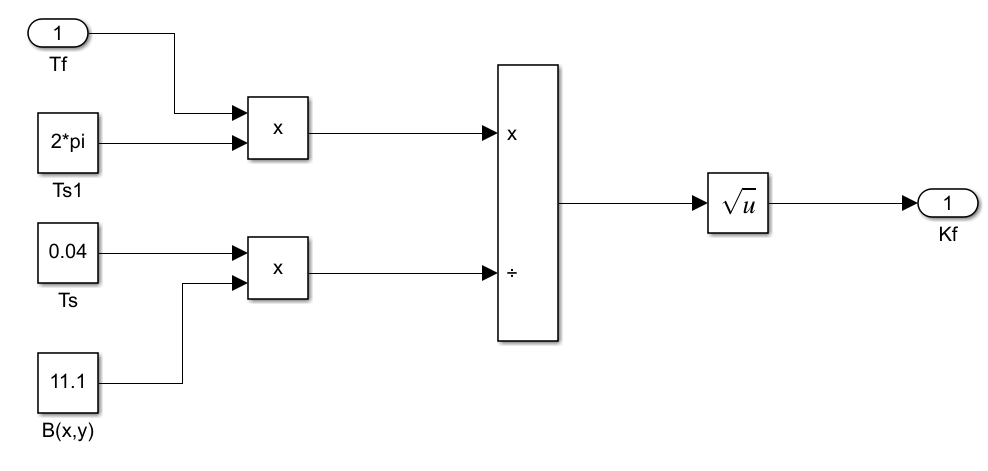
\includegraphics[width=\textwidth]{Figuras/Teorico/GanhoDoFiltro_Kf.png}
    \label{fig:coeficienteKf}
    
\end{figure}

Aqui, \(B(x, y)\) representa a função beta de Euler, um componente crucial que desempenha um papel na normalização do filtro em relação à distribuição de frequências.

Um aspecto crucial relacionado ao ganho \(K_f\) é que ele precisa ser calculado de maneira a preservar o desvio padrão do sinal de saída como unitário. A frequência de amostragem \(T_s\) definida neste estudo é 0.04 segundos.

O ruído utilizado para excitação do filtro é dado pelas equações utilizadas no vento turbulento (\ref{eq:ventoTurbulento}) e vento ondulante (\ref{eq:ventoOndulante}), assim o ruído é dado por:

\begin{equation}
r = \sqrt{-2 \ln(x_1)} \sin(2\pi x_2)
\label{eq:ruidogaussiano}
\end{equation}
e representado na figura \ref{fig:RuidoGaussiano}.

\begin{figure}[h]
    \centering
    \caption{O ruído utilizado para ativar o filtro gerado no \textit{software} MATLAB/SIMULINK}
    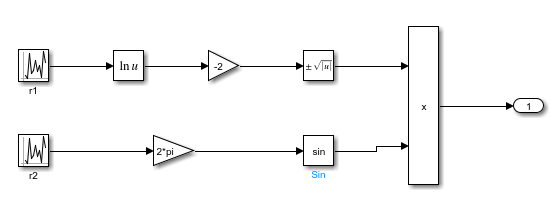
\includegraphics[width=0.8\textwidth]{Figuras/Teorico/ruidoGaussiano.png}
    \label{fig:RuidoGaussiano}    
\end{figure}

Este ruído, tem um desvio padrão unitário e segue uma distribuição gaussiana, e é gerado a partir de duas variáveis aleatórias \(x_1\) e \(x_2\), ambas com distribuição uniforme no intervalo de 0 a 1. Esse método de geração de ruído é fundamental para simular com precisão a natureza aleatória e estocástica da turbulência do vento em modelos de séries temporais.

O desvio padrão da turbulência \(D_p\) varia em função do coeficiente de turbulência longitudinal \(K_p\) e da velocidade média do vento \(v\), seguindo a relação
\begin{equation}
D_p(v_t) = K_p v
\end{equation}

O coeficiente \(K_p\), também chamado de fator de turbulência, é determinado pelas características específicas do terreno. Conforme \citeonline{stannard2007performance}, foram compilados valores estimados para \(K_p\) para diversos tipos de terreno demonstrados na Tabela \ref{tab:fator de turbulencia}

    \begin{table}[h]
        \caption{Fatores de turbulência para diferentes terrenos}
        \centering
        \begin{tabular}{c|c}
        \hline
        Tipo de Terreno & \(K_p\) \\
        \hline
        Áreas Litorâneas & 0.123 \\
        Lagos & 0.145 \\
        Lugares Abertos & 0.189 \\
        Áreas em construção & 0.285 \\
        Centros Urbanos & 0.434 \\
        \hline
        \end{tabular}
        \label{tab:fator de turbulencia}
        \fonte{Adaptado de \citeonline{koch2010}}
    \end{table}

\par Esta tabela é essencial para entender como variáveis ambientais influenciam a turbulência do vento em diferentes locais. Assim, adotando todas as equações e fatores topográficos, tem-se o modelo da serie temporal no MATLAB/SIMULINK representando na Figura \ref{fig:SérieTemporal} e a serie temporal gerada na Figura \ref{fig:SérieTemporal_resultado}.

    \begin{figure}[h]
        \centering
        \caption{Série Temporal de Vento modelado no \textit{software} MATLAB/SIMULINK}
        \includegraphics[width=1\textwidth]{Figuras/Teorico/SerieTemporaldeVento.png}
        \label{fig:SérieTemporal}    
    \end{figure}
    
    \begin{figure}[h]
        \centering
        \caption{Resultado do modelo da Série Temporal de Vento \textit{software} MATLAB/SIMULINK}
        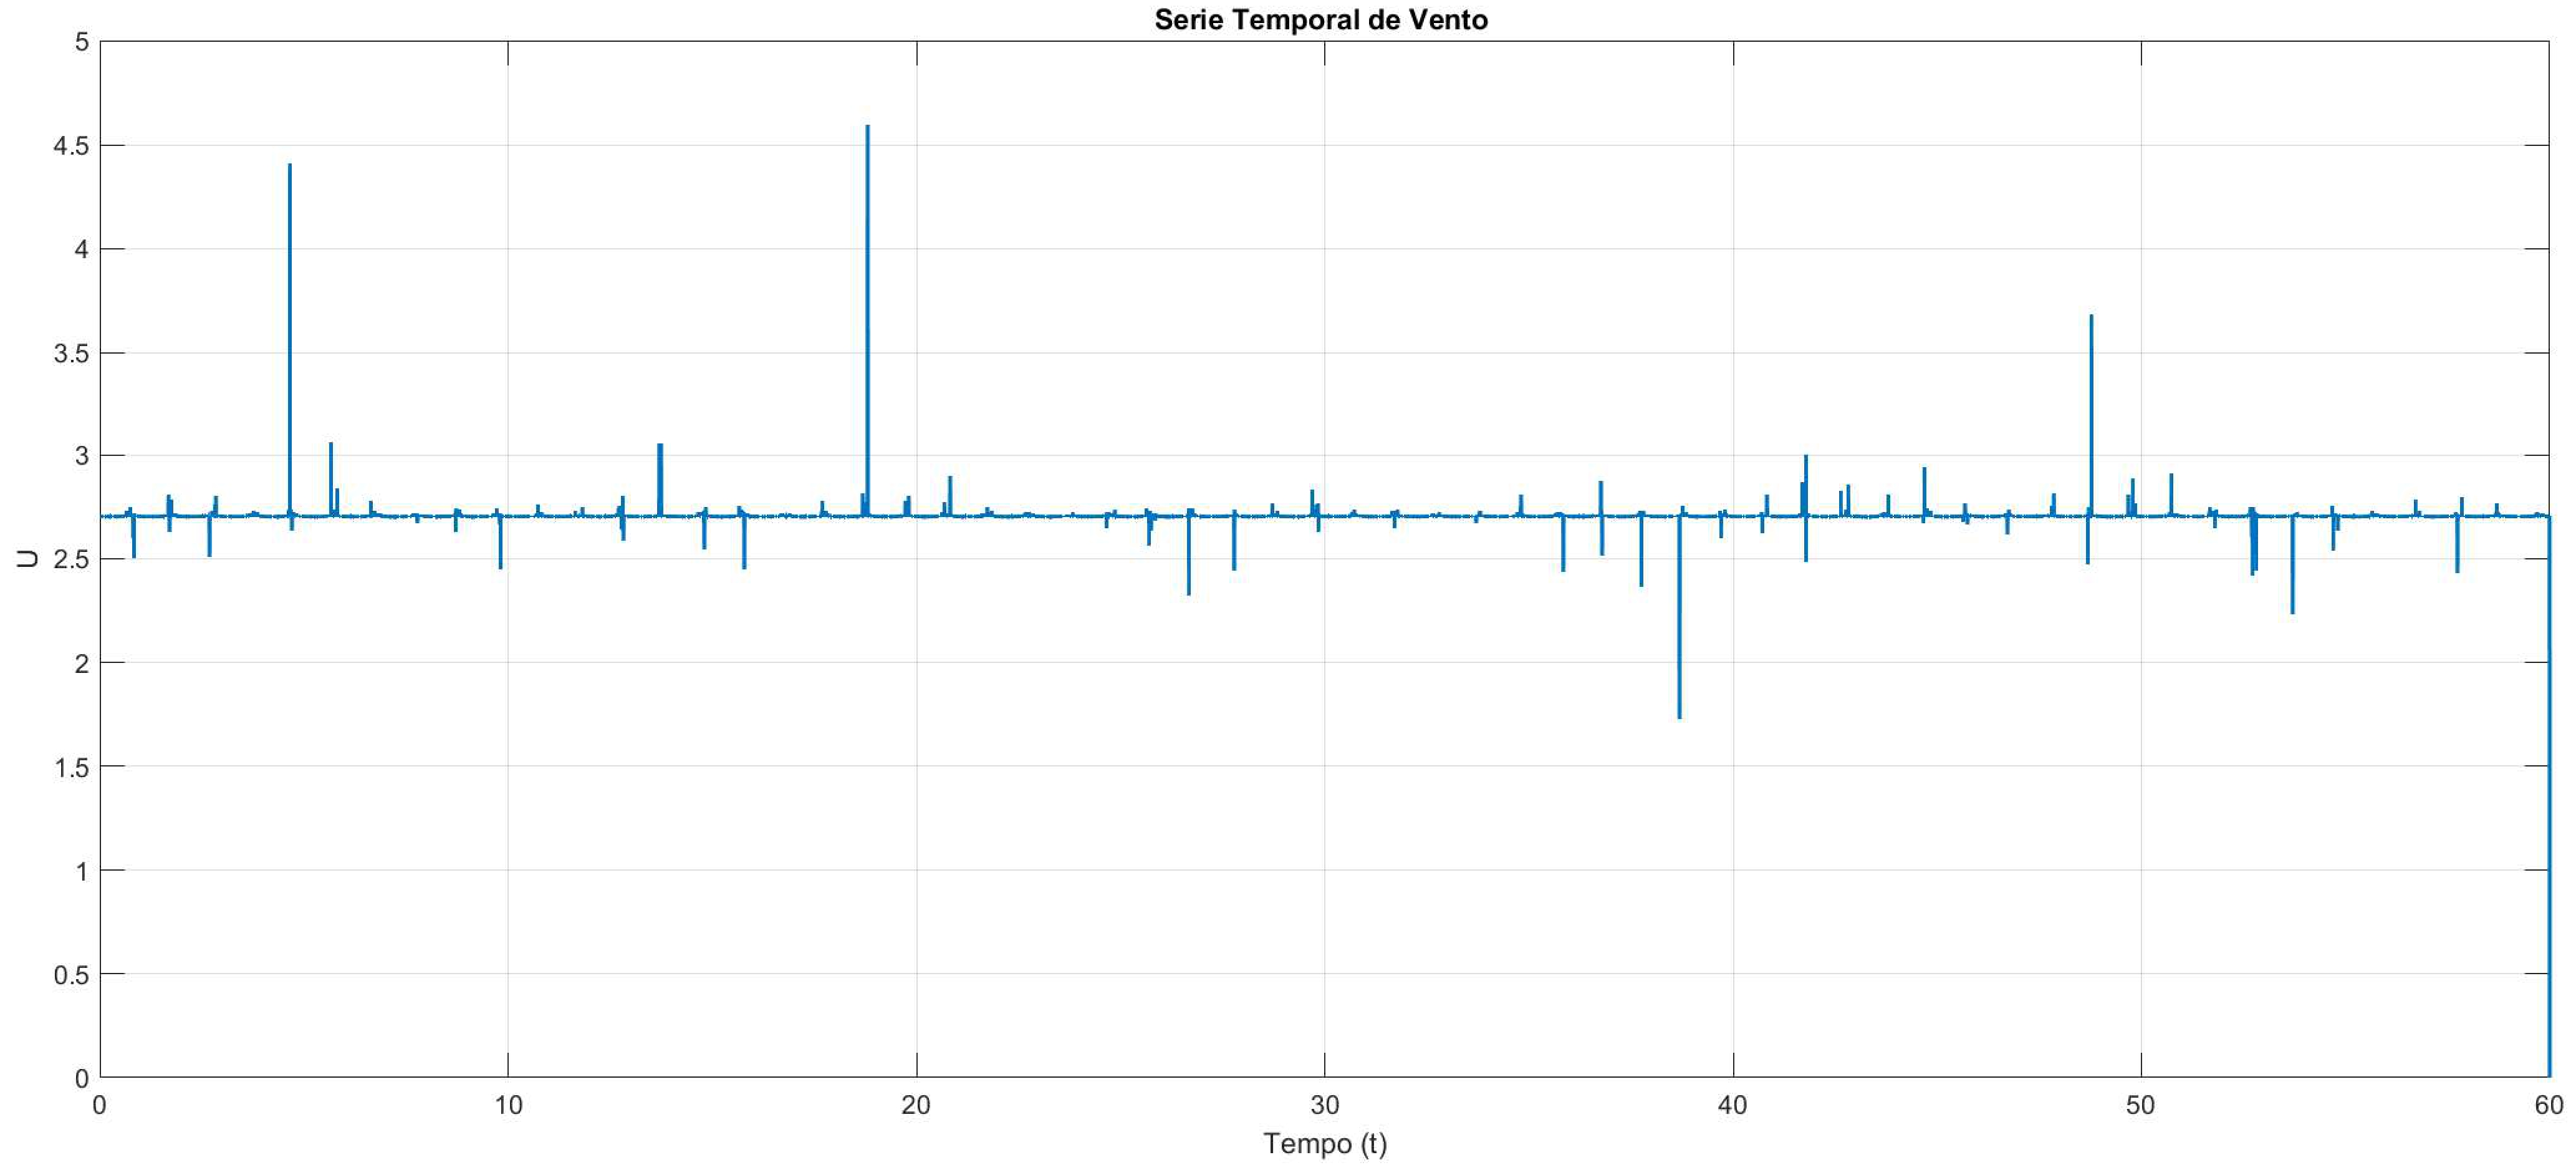
\includegraphics[width=1\textwidth]{Figuras/Teorico/serie temporal de vento_.png}
        \label{fig:SérieTemporal_resultado}    
    \end{figure}







%\section{Aspectos Técnicos dos Aerogeradores}


%\section{Conceitos básicos de energia eólica}

\section{Princípios de fundamento das turbinas eólicas} % Analisar esse tópico
\par As turbinas eólicas, comumente conhecidas como aerogeradores, são dispositivos projetados para otimizar a captação da energia cinética do vento, transformando-a em energia elétrica utilizável. O processo de conversão inicia-se quando o vento interage com as pás do rotor, que giram devido à força do vento. Essa rotação segue o princípio da conservação de energia, convertendo a energia cinética em energia mecânica no rotor, que, por sua vez, é transmitida ao gerador elétrico.

\par Na figura \ref{fig:EsquemaAbregenteOperacao}, observa-se um esquema detalhado desse processo. O vento impulsiona as pás da turbina, gerando energia mecânica que é transmitida por meio de um multiplicador mecânico, responsável pela conversão de torque e velocidade. Essa energia mecânica elevada é então convertida em energia elétrica no gerador. A conversão de energia mecânica em elétrica é acompanhada por um sistema de controle e proteção eletrônica, garantindo a segurança e eficiência da operação. Em seguida, um transformador elevador ajusta a tensão da energia gerada para níveis compatíveis com a rede elétrica, facilitando a distribuição.

    \begin{figure}[H]
        \caption{Esquema abrangente de operação de um aerogerador.}
        \label{fig:EsquemaAbregenteOperacao}
        \centering
        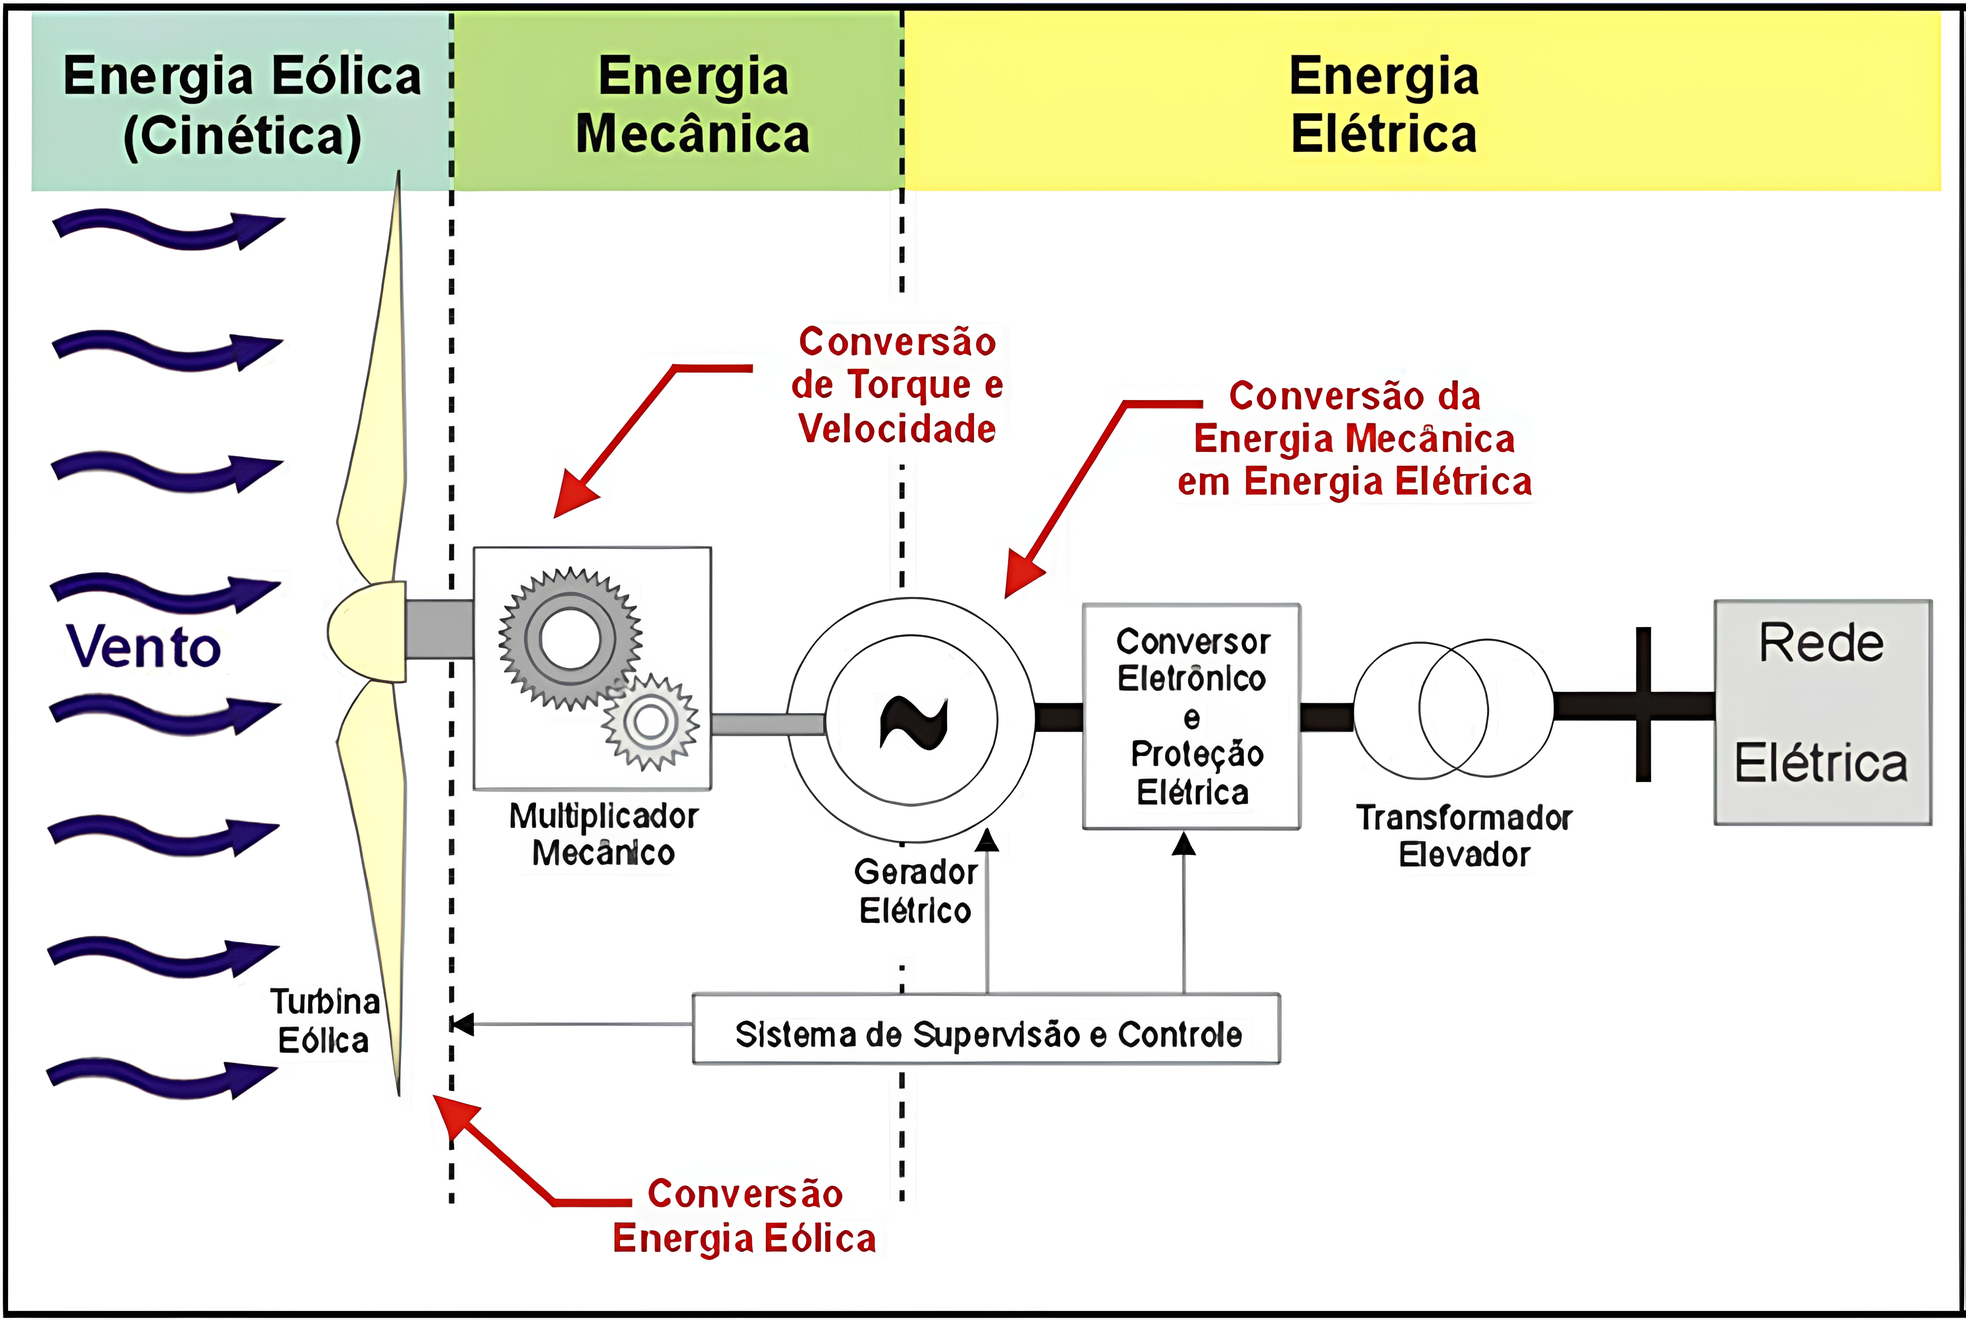
\includegraphics[width=0.8\textwidth]{Figuras/Teorico/Esquema geral de funcionamento de um aerogerador.png}
        \fonte{\citeonline{pavinatto2005}}
    \end{figure}

\par Historicamente, diversos tipos de turbinas foram experimentados, incluindo configurações de eixo horizontal e vertical, com várias quantidades de pás. Contudo, para geração em grande e médio porte, predominam atualmente as turbinas de eixo horizontal, com estrutura robusta, três pás e geradores de indução, que também possuem alinhamento ativo, como exemplificado na imagem \ref{fig:EsquemaTurbina}. Apesar de sua popularidade, algumas características dessas turbinas, como o controle do ângulo de passo, ainda são alvo de discussões técnicas e ajustes para aprimorar a eficiência da captação de energia e a resposta às condições variáveis do vento.

\par Além disso, existem vários aspectos que caracterizam um aerogerador, entre eles a topologia, o tamanho, o nível de potência, a eficiência energética e a localização.



\section{Componentes de Aerogerador de Eixo Horizontal}  

\par Os aerogeradores de eixo horizontal são os mais comuns e amplamente utilizados no setor de energia eólica devido à sua eficiência e capacidade de gerar grandes quantidades de energia. A estrutura básica de um aerogerador de eixo horizontal é composta por diversos componentes essenciais que trabalham em conjunto para converter a energia cinética do vento em energia elétrica.

\begin{figure}[H]
    \caption{Esquema de Turbina Eólica Moderna.}
    \label{fig:EsquemaTurbina}
    \centering
    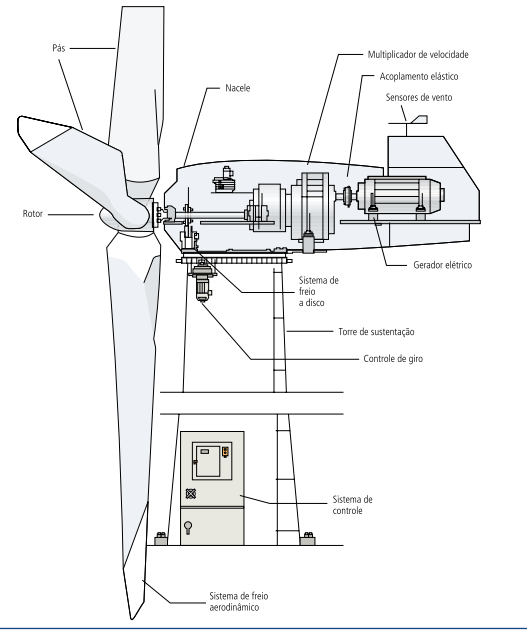
\includegraphics[width=0.6\textwidth]{Figuras/Teorico/Construtivos.png}
    \fonte{\citeonline{site:CBEE}}
\end{figure}



\begin{enumerate}[label=\Roman*,start=1]
    \item Pás: Ou lâminas, utilizando os mesmos perfis aerodinâmicos das asas de aviões, elas captam a energia cinética produzida pelos ventos e transferem para o rotor. Compostas geralmente de materiais leves e resistentes, como fibra de vidro ou carbono.
    \item Rotor: Composto pelas pás e pelo cubo do rotor, o rotor é responsável por converter a energia cinética do vento em energia mecânica.
    \item Nacele: É o compartimento instalado no alto da torre, sendo ele o responsável por abrigar, suportar e proteger os principais componentes do sistema de geração de energia, como gerador, eixo e demais acoplamentos (de acordo com a configuração).
    \item Multiplicador de velocidade: Ou caixa de engrenagens. Utilizado em sistema com geradores assíncronos, sua principal funcionalidade é transformar uma rotação lenta em uma rotação rápida, geralmente de um intervalo de 10-60 rpm para valores próximos a 1200-1800 rpm.  
    \item Acoplamento elástico: É um tipo de acoplamento utilizado para conectar eixos rotativos. Sua função é transmitir o torque de um eixo a outro, absorvendo choques, vibrações e desalinhamento.
    \item Gerador Elétrico: Responsável pela conversão de energia mecânica em energia elétrica. Sendo mais comumente utilizado gerador de indução \cite{ackermann2005}.
    \item Sensores de vento: Esses sensores monitoram as condições do vento, medindo a velocidade e a direção, por sua vez, comunicando ao mecanismo de orientação direcional.
    \item Controle de giro: Também conhecido como sistema de \textit{yaw}, é o componente responsável pelo posicionamento da nacele, alinhando-a em direção do vento e maximizando a captação.
    \item Torre de sustentação: Estrutura vertical responsável por suporta a nacele e o rotor, permitindo a captação dos ventos em uma altura maior. 
    \item Sistema de Freio: O sistema de freio é empregado para parar ou controlar a rotação do rotor em condições específicas, como durante a manutenção, em situações de emergência ou quando há vento excessivo.
    \item Sistema de controle: Responsável por garantir a segurança e otimizar a potência gerada através do controle de rotação, acionamento dos freios e/ou controle de passo. Além de, garantir a qualidade da energia gerada.
\end{enumerate}
\section{Perfil Aerodinâmico}
    \par O perfil aerodinâmico das pás de um aerogerador desempenha um papel fundamental na eficiência e na capacidade de geração de energia do sistema. As pás dos aerogeradores são projetadas para transformar a energia cinética do vento em energia mecânica de rotação, que, por sua vez, é convertida em eletricidade pelo gerador. Para maximizar a eficiência dessa conversão, é essencial que o design do perfil das pás considere uma série de fatores aerodinâmicos, como a forma e o ângulo de ataque da superfície, a curvatura e o alongamento.

    \par Um bom projeto de perfil aerodinâmico visa maximizar o coeficiente de sustentação e minimizar o coeficiente de arrasto em uma ampla faixa de velocidades de vento e ângulos de operação. Esse equilíbrio entre sustentação e arrasto é crucial, pois permite que as pás gerem a força de rotação necessária com menor resistência, contribuindo para uma maior eficiência energética do aerogerador, como destacado na figura \ref{fig:Aspectos de um perfil aerodinâmico.}. Além disso, o perfil deve ser resistente a condições extremas e oferecer boa resposta a variações de intensidade e direção do vento, otimizando o desempenho e a durabilidade do aerogerador.

        \begin{figure}
            \centering
            \caption{Aspectos de um perfil aerodinâmico.}
            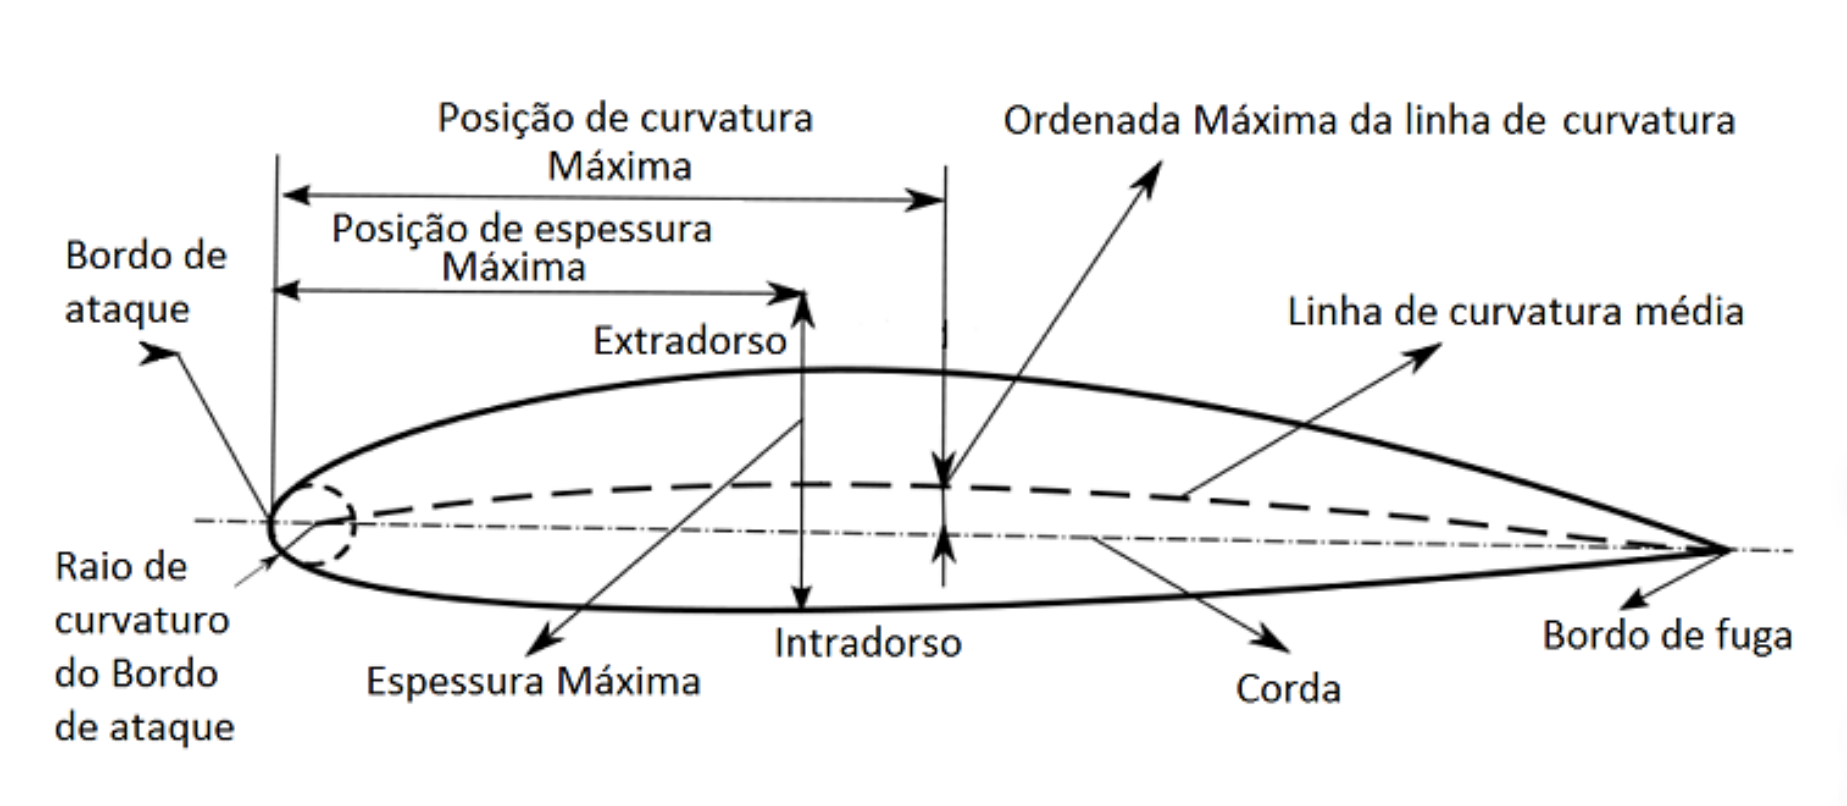
\includegraphics[width=0.7\linewidth]{Figuras//Teorico/PerfilAerodinamico01.png}
            \label{fig:Aspectos de um perfil aerodinâmico.}
            \fonte{\citeonline{junior2012desempeno}}
        \end{figure}
        
        \begin{itemize}  
            \item \textbf{Bordo de Ataque e Bordo de Fuga:}   
            Referem-se, respectivamente, aos pontos dianteiro e traseiro do aerofólio. O bordo de ataque é o ponto inicial de contato do ar com o perfil, enquanto o bordo de fuga é o ponto final, onde o ar se desprende da superfície do aerofólio.  
            
            \item \textbf{Extradorso e Intradorso:}   
            Estas são as superfícies externas do aerofólio, sendo o extradorso a superfície superior e o intradorso a superfície inferior, que se estendem do bordo de ataque até o bordo de fuga.  
            
            \item \textbf{Linha de Corda:}   
            Trata-se de uma linha imaginária que conecta o bordo de ataque ao bordo de fuga. Essa linha serve como referência para a análise de diversos parâmetros geométricos e aerodinâmicos do aerofólio.  
            
            \item \textbf{Corda:}   
            Corresponde ao comprimento do segmento de reta que une os pontos do bordo de ataque e do bordo de fuga. É uma medida fundamental na caracterização geométrica do aerofólio e influencia diretamente suas propriedades aerodinâmicas.  
            
            \item \textbf{Linha de Curvatura:}   
            Refere-se ao lugar geométrico dos pontos equidistantes entre o extradorso e o intradorso, medidos perpendicularmente à linha de corda. A linha de curvatura define a forma média do aerofólio, sendo útil para determinar o comportamento aerodinâmico e o perfil de pressão ao longo do aerofólio.  
            
            \item \textbf{Camber:}   
            Denomina-se "camber" à assimetria entre as superfícies superior (extradorso) e inferior (intradorso) de um aerofólio. Essa assimetria é responsável por gerar sustentação, uma vez que altera a distribuição de pressão ao redor do perfil.  
        \end{itemize}  
        
    \subsection{Coeficientes e Parâmetros Aerodinâmicos}
        \par Quando um perfil aerodinâmico é imerso em um escoamento de fluido, o ar (ou outro fluido) que se movimenta em sua direção se divide em duas correntes principais. Como pode ser visto na figura \ref{fig:Escoamento_ao_longo_do_perfil}, uma dessas correntes passa sobre a superfície superior do perfil, conhecida como \textbf{extradorso}, enquanto a outra corrente circula pela superfície inferior, chamada \textbf{intradorso}.

        \begin{figure}
            \centering
            \caption{Escoamento ao longo do perfil.}
            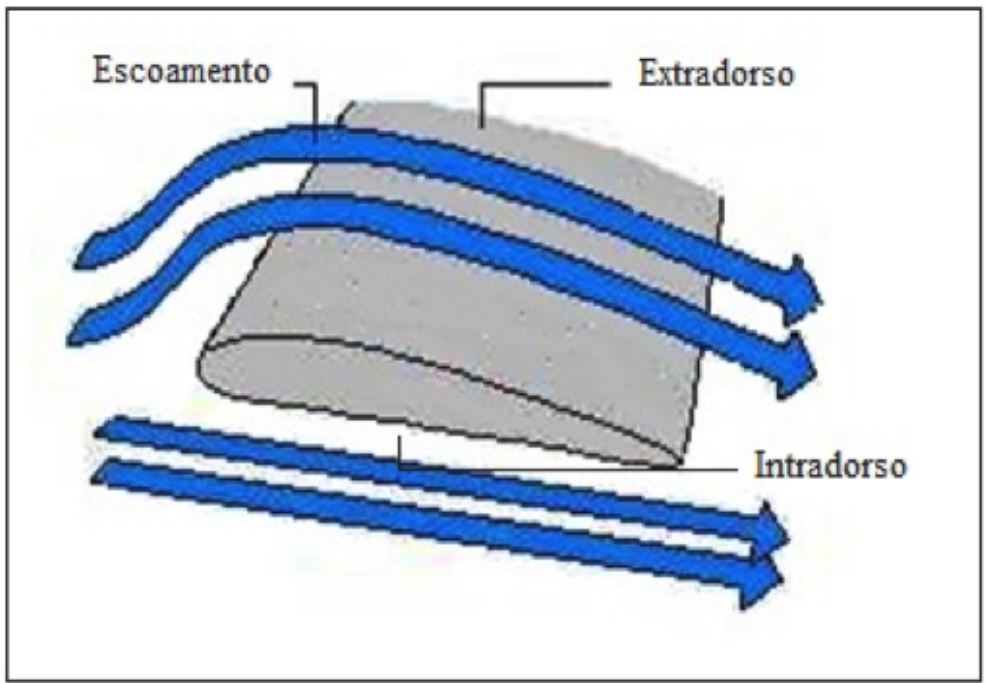
\includegraphics[width=0.5\linewidth]{Figuras//Teorico/EscoamentoCirculandoOPerfil.png}
            \label{fig:Escoamento_ao_longo_do_perfil}
            \fonte{\citeonline{peixoto2009nocao}}
        \end{figure}

        \par Essa divisão do fluxo de ar ao redor do perfil cria diferenças de pressão entre o extradorso e o intradorso. Normalmente, devido à curvatura do perfil, o fluido que passa pelo extradorso se move mais rapidamente do que aquele que passa pelo intradorso. Segundo o princípio de Bernoulli, essa diferença de velocidade gera uma pressão menor no extradorso em comparação ao intradorso, resultando em uma força de sustentação que age sobre o perfil e uma força de arrasto que age perpendicular a ela, como pode ser visualizado na figura \ref{fig:Forças_Aerodinâmicas}.

        \begin{figure}
            \centering
            \caption{Forças Aerodinâmicas}
            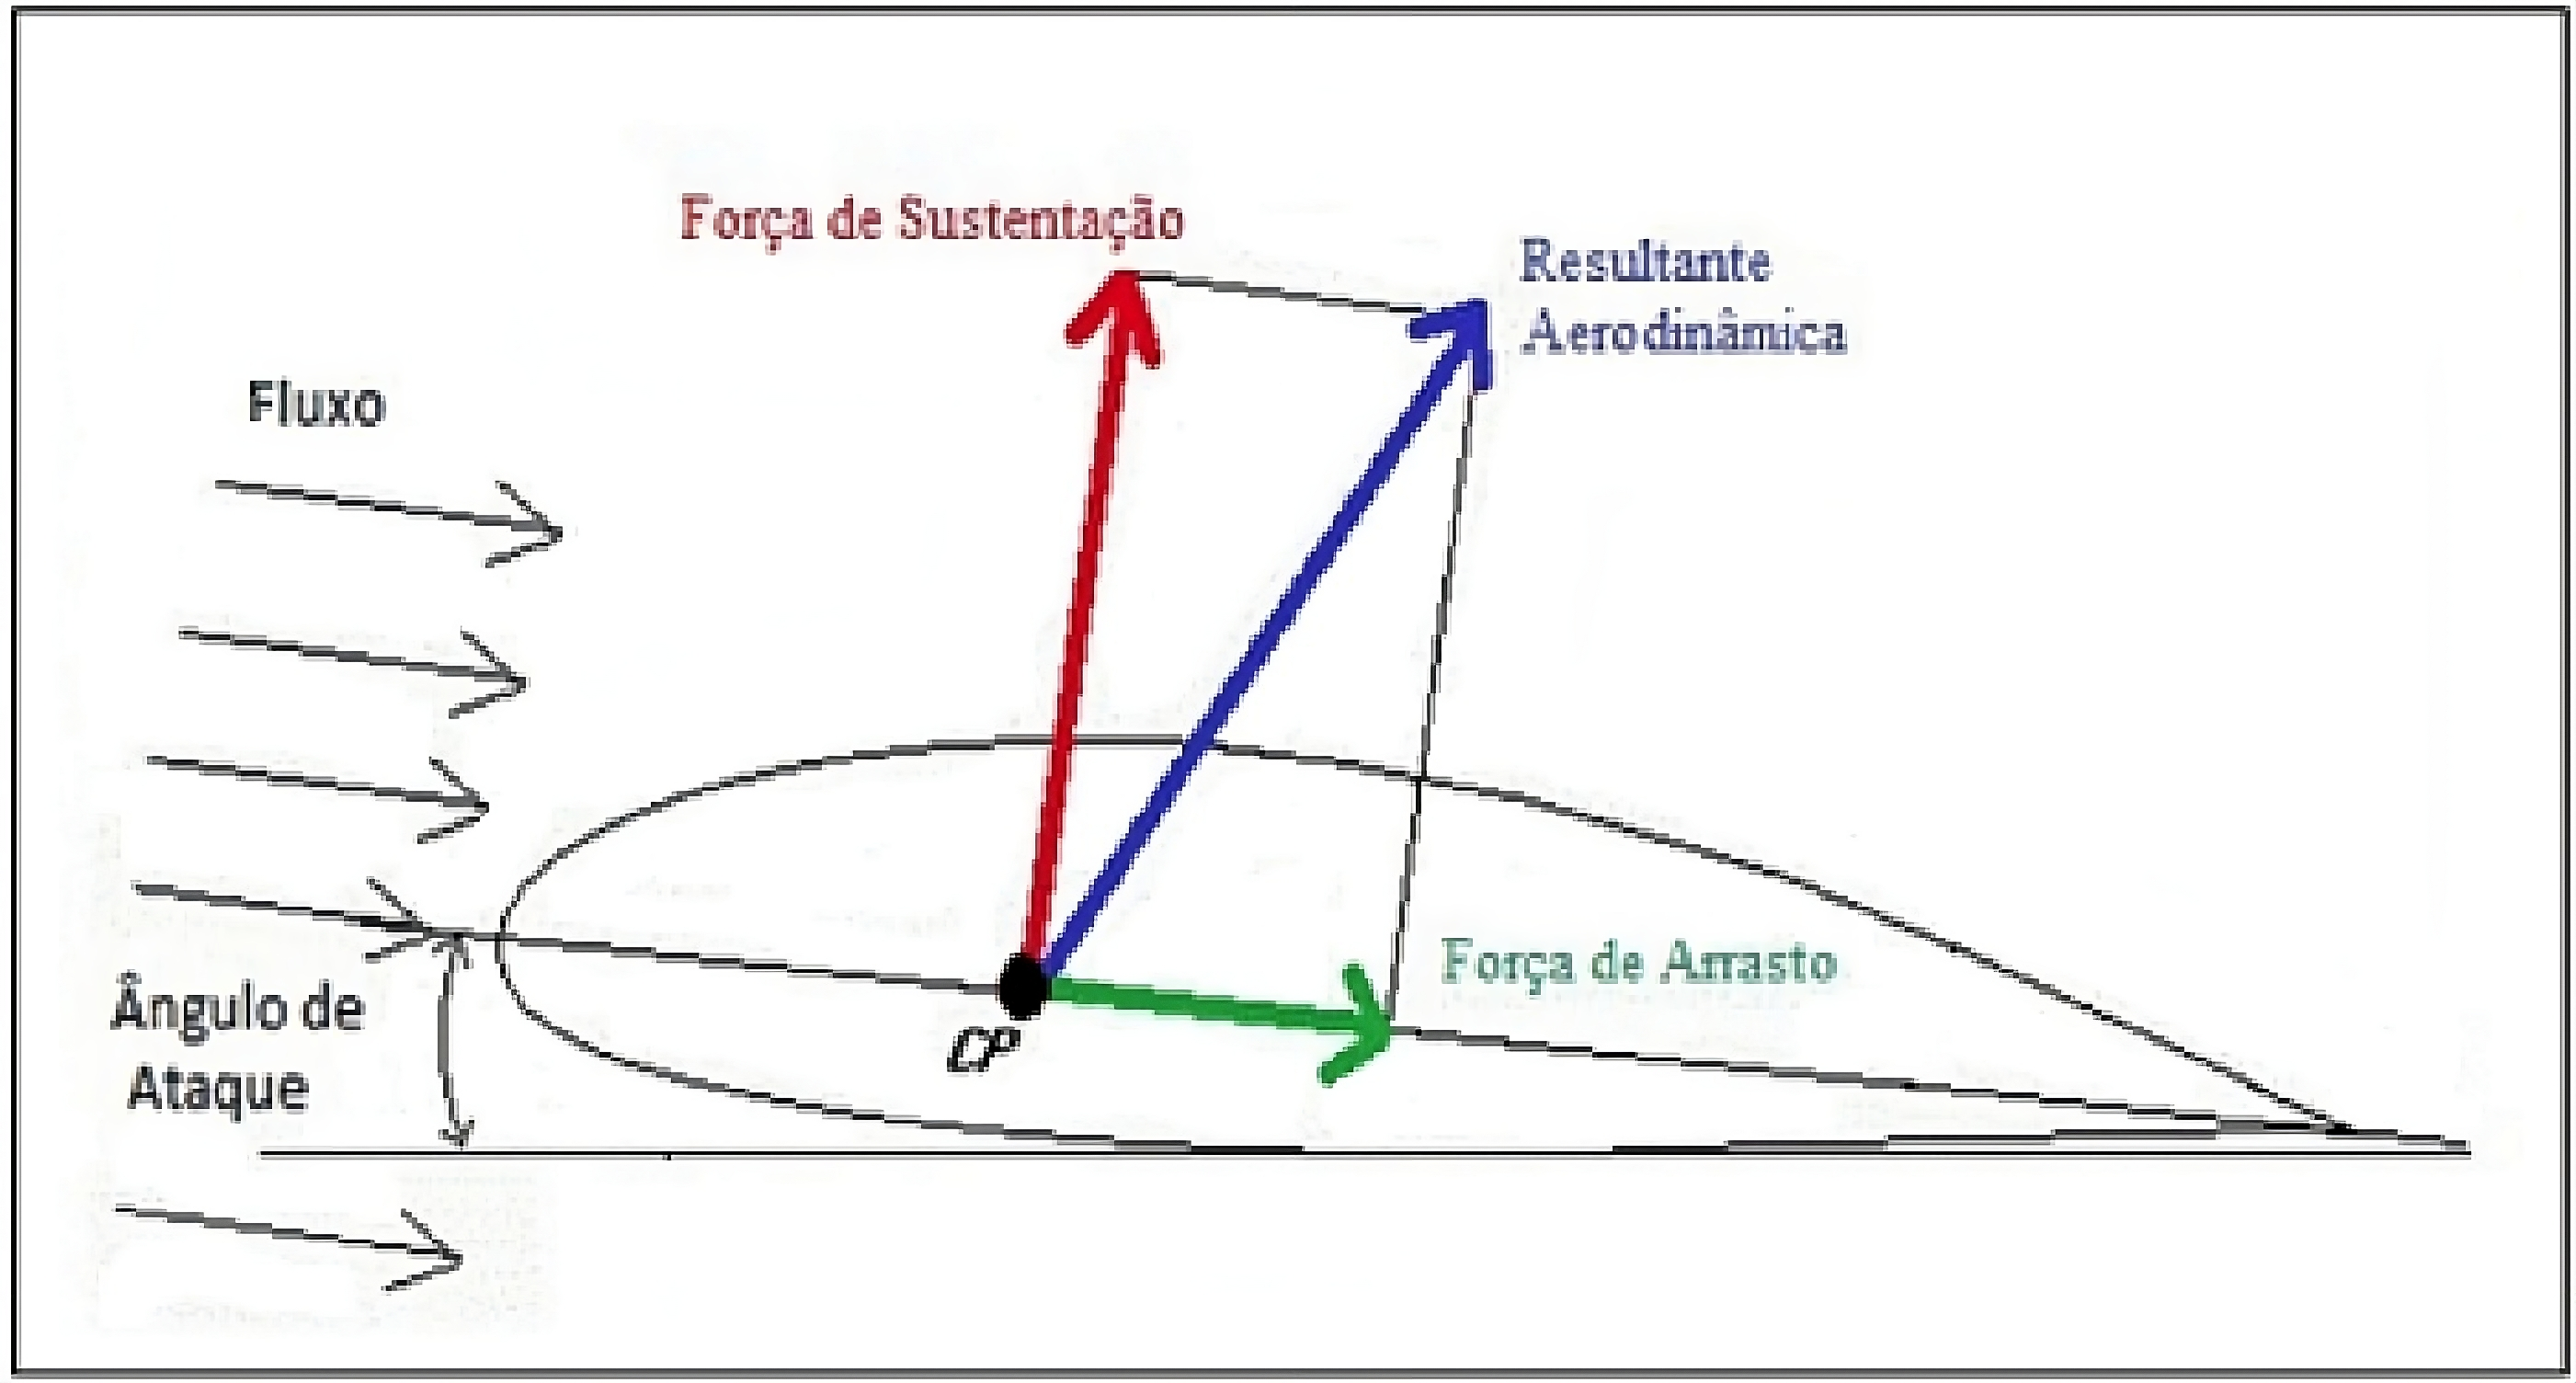
\includegraphics[width=0.8\linewidth]{Figuras//Teorico/Esforços Aerodinâmicos.png}
            \fonte{\citeonline{weltner2001dinamica}}
            \label{fig:Forças_Aerodinâmicas}
        \end{figure}

        \par Para calcular a Força de Sustentação \textbf{\( L  \)} e Força de Arrasto \textbf{\( D \)} em um perfil aerodinâmico, utiliza-se repectivamente a Equação \ref{eq:Força de Sustentação L} e \ref{eq:Eq Força de Arrasto}, conforme descrito por \citeonline{halliday1996fundamentos}:

        \begin{equation}
        L = \frac{1}{2} \cdot \rho \cdot V^2 \cdot A_S \cdot C_L 
        \label{eq:Força de Sustentação L}
        \end{equation}

        \begin{equation}
        D = \frac{1}{2} \cdot \rho \cdot V^2 \cdot A_S \cdot C_D
        \label{eq:Eq Força de Arrasto}
        \end{equation}
        
        Em que:
        \begin{itemize}  
            \item $\rho$: representa a densidade do fluido ao redor do perfil;  
            \item $V$: é a velocidade relativa do escoamento;  
            \item $A_s$: é a área de superfície do perfil;  
            \item $C_L$: é o coeficiente de sustentação, que depende da forma e do ângulo de ataque do perfil.
            \item $C_D$: é o coeficiente de Arrasto, que indica a resistência ao movimento do perfil dentro do fluido.
        \end{itemize}   

        \par Essa expressão demonstra que a força de sustentação aumenta com a densidade do fluido, com o quadrado da velocidade do escoamento e com o coeficiente de sustentação, que reflete as características aerodinâmicas do perfil. Quanto maior o coeficiente de sustentação, maior a capacidade do perfil de gerar sustentação.

        \par Por outro lado, a Força de Arrasto atua paralelamente à direção do fluxo e se opõe ao movimento do perfil no escoamento. Essa força é resultado da interação entre o aerofólio e o fluido, e está relacionada principalmente a duas causas: o arrasto de atrito e o arrasto de forma.

        \begin{itemize}  
            \item \textbf{Arrasto de Atrito:} Esse tipo de arrasto ocorre devido às tensões de cisalhamento na superfície do perfil, geradas pela fricção entre o fluido e a superfície do objeto.  
    
            \item \textbf{Arrasto de Forma:} Esse tipo de arrasto é causado pelo desequilíbrio de pressão em torno do perfil, especialmente nas regiões onde o fluxo se separa da superfície.  
        \end{itemize}  




        
\section{Controle de Ângulo de Passo}
\section{Controlador Yaw}

\section{Turbina Eólica TE24}
    \par Para o desenvolvimento deste trabalho, foi utilizada a turbina eólica TE24, produzida pela VIND Aerogeradores. Ela se destaca por sua tecnologia totalmente nacional, facilitando o suporte técnico e a manutenção local. Este aerogerador é projetado para maximizar a eficiência e a flexibilidade operacional, incorporando técnicas e tecnologias geralmente aplicadas apenas a aerogeradores de grande porte.
    
    \par Desenvolvida em parceria com o Instituto Tecnológico de Aeronáutica (ITA), a turbina apresenta variadores de passo eletronicamente controlados e sistemas de controle de última geração, garantindo alta eficiência e adaptabilidade a diferentes condições de vento.

    \par A TE24 é equipada com um rotor de 15 metros de diâmetro e possui uma potência nominal de 24KW, capaz de gerar eletricidade suficiente para atender a demanda de pequenos empreendimentos comerciais ou unidades industriais. A turbina opera eficientemente em uma ampla variação de velocidade de vento, indo de 2,3 m/s (velocidade de \textit{cut-in}) até 20 m/s (velocidade de \textit{cut-out}). Essa faixa operacional ampla permite aplicabilidade em diversas regiões, adaptando-se a diferentes perfis de vento. Essa característica é destacada nos dados obtidos da operação em Franca-SP, detalhados na Tabela \ref{tab:GeraçãoDiferentesVel_TE24}.

    \begin{table}[h]
        \caption{Comparação entre geração estimada com dados teóricos e dados reais de geração de energia eólica na Vila Santa Terezinha, Franca – SP.}
        \centering
        \resizebox{\textwidth}{!}{ % Ajusta a tabela para a largura da página
        \begin{tabular}{|c|c|c|c|}
            \hline
            \textbf{Vel. Média de Vento ($\frac{m}{s}$)} & \textbf{Geração estimada com dados teóricos ($\frac{kwh}{mês}$)} & \textbf{Geração estimada com dados reais ($\frac{kwh}{mês}$)} & \textbf{\%} \\ \hline
            3   & 1150  & 1808  & 57\% \\ \hline
            3.5 & 1871  & 2722  & 45\% \\ \hline
            4   & 2748  & 3729  & 36\% \\ \hline
            4.5 & 3727  & 4776  & 28\% \\ \hline
            5   & 4748  & 5817  & 23\% \\ \hline
            5.5 & 5763  & 6817  & 18\% \\ \hline
            6   & 6736  & 7753  & 15\% \\ \hline
            6.5 & 7642  & 8610  & 13\% \\ \hline
            7   & 8469  & 9381  & 11\% \\ \hline
            7.5 & 9206  & 10061 & 9\%  \\ \hline
            8   & 9848  & 10645 & 8\%  \\ \hline
        \end{tabular}
        }
        \label{tab:GeraçãoDiferentesVel_TE24}
        \fonte{Dados de Geração TE24 - Real - Franca}
    \end{table}    


    \par A turbina eólica TE24 é projetada para operar de forma eficiente e durável, incorporando materiais de alta qualidade. As pás são feitas de compósitos reforçados com fibras de vidro, garantindo durabilidade e resistência. A torre é galvanizada a fogo com tripla camada de proteção contra corrosão, aumentando a vida útil do equipamento. A tensão de saída da turbina pode ser configurada para 220V, 380V ou 440V trifásica, conforme as necessidades da instalação. Suas característica técnicas elétricas estão descritas na tabela \ref{tab:TE24_DadosTecnicos_Eletrica}.

    \begin{table}[h]
        \centering
        \caption{Características Elétricas do Aerogerador TE24}
        \begin{tabular}{|l|l|}
            \toprule
            \textbf{Característica}                  & \textbf{Descrição}                                  \\ \midrule
            Potência nominal do gerador              & 30 KVA ou 24KW                                      \\
            Tensão de saída                          & 220/380/440V trifásica                              \\
            Velocidade nominal do vento              & 09 m/s                                              \\
            Velocidade mínima                        & 2,3 m/s (“cut-in”)                                  \\
            Velocidade máxima de operação            & 20,0 m/s (“cut-out”)                                \\
            Velocidade de proteção                   & 45,0 m/s (rajada)                                   \\
            Controle de prioridades de carga         & 4 ramais                                            \\
            Inversor de Frequência                   & Versão “ON GRID” ou similar                         \\ \bottomrule
        \end{tabular}
        \label{tab:TE24_DadosTecnicos_Eletrica}
    \end{table}
    
    \par Além disso, a turbina TE24 oferece flexibilidade na instalação, podendo ser configurada para diferentes alturas de torre e tipos de solo. A possibilidade de conexão on-grid permite a compensação da energia gerada com o consumo, reduzindo significativamente os custos de eletricidade e aumentando a viabilidade econômica do projeto. Suas característica técnicas construtivas estão descritas na tabela \ref{tab:TE24_DadosTecnicos_Construtivos}.

     \begin{table}[h]
        \centering
        \caption{Características Construtivas do Aerogerador TE24}
        \begin{tabular}{|l|l|}
        \toprule
        \textbf{Característica}                  & \textbf{Descrição}                                  \\ \midrule
        Tipo de turbina                          & Três pás                                            \\
        Posição do eixo                          & Horizontal                                          \\
        Diâmetro do rotor                        & 15 metros                                           \\
        Variador de Passo de hélice              & Ativo – mecanismo original                           \\
        Movimento Azimutal (“yaw”)               & Ativo                                               \\
        Material das pás                         & Compósitos                                          \\
        Torre – configuração                     & Chapa dobrada e galvanizada a fogo                  \\
        Proteção contra corrosão                 & Tripla camada                                       \\
        Altura da torre                          & Variável de acordo com o local escolhido            \\
        Sistema de aterramento da torre          & Sim                                                 \\
        Sistema de freio de emergência           & Sim                                                 \\ \bottomrule
        \end{tabular}
        \label{tab:TE24_DadosTecnicos_Construtivos}
    \end{table}
\par Devido às diversas características presentes neste modelo de aerogerador, ele foi escolhido como referência para o desenvolvimento deste trabalho. Suas propriedades construtivas, incluindo o controle do ângulo de passo da hélice, permitem a análise da máxima potência. As características elétricas, como a velocidade de \textit{cut-in} de 2,3 m/s, conferem alta aplicabilidade em cenários adversos, tornando este modelo uma excelente opção para o estudo e desenvolvimento propostos.


%\section{Mecanismos de Controle de Passo}
%    \subsection{Controle de Passo Variável}
%    \subsection{Controle de Passo Coletivo vs Individual}
%\section{Modos de Operação da Turbina}
%    \subsection{Modo de Potência Constante}
%    \subsection{Modo de Velocidade Variável}
%    
%    \section{Turbinas de velocidade variável}
%        \subsection{Vantagens}
%        \subsection{Desafios}
%        \subsection{Aplicações}
%    
%    \section{Modelagem da Turbina Eólica}
%        \par  Desenvolvimento do modelo matemático da turbina eólica de velocidade variável. Consideração dos componentes principais: pás, gerador, conversor de frequência, etc. Implementação do modelo no MATLAB Simulink.
%        \subsection{Equações de Movimento}
%        \subsection{Modelo de Pás}
%        \subsection{Modelo do Gerador}
    